\documentclass[12pt, times new roman]{article}
\usepackage[utf8]{inputenc}
\usepackage{graphicx}
\usepackage{float}

\title{Hasil Resume Oracle Application Express}
\author{Yusuf Jordan El Anwar}
\date{October 2019}

\begin{document}

\maketitle
\section{Low Code Application Development}
Low-code adalah sebuah cara untuk membuat dan mendesain sebuah aplikasi dengan cepat walaupun dalam membuat kode masih secara manual.Dengan bantuan Low-code memiliki ui yang berbasis grafik dalam mengatur dan menata sebuah aplikasi sehinggan pengembang aplikasi dapat menyelesaikan aplikasi dengan cepat.
\subsection{Membuat Aplikasi dengan low-code}
\begin{itemize}
\item Masuk ke situs Apek oracle.Login ke akun oracle Anda, jika belum memiliki akun silahkan daftar.
\begin{figure}[!htbp]
	\centering
	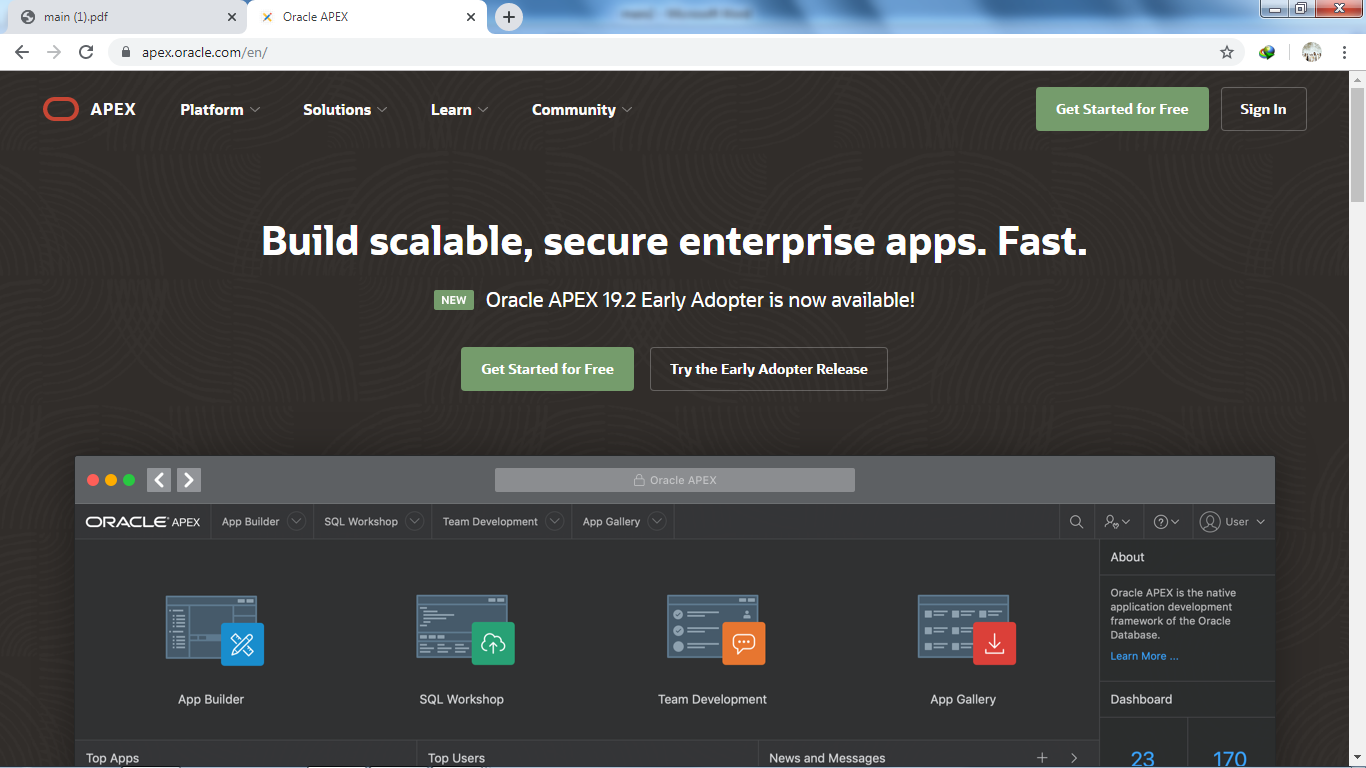
\includegraphics[width=10cm]{figures/Screenshot_1.png}
	\caption{Login}
\end{figure}
\item Untuk membuat aplikasi.Karena Masih belajar Kita Pake Aplikasi yang telah di sediakan oleh oracle. Klik App Builder - Create - From a File 
\begin{figure}[!htbp]
	\centering
	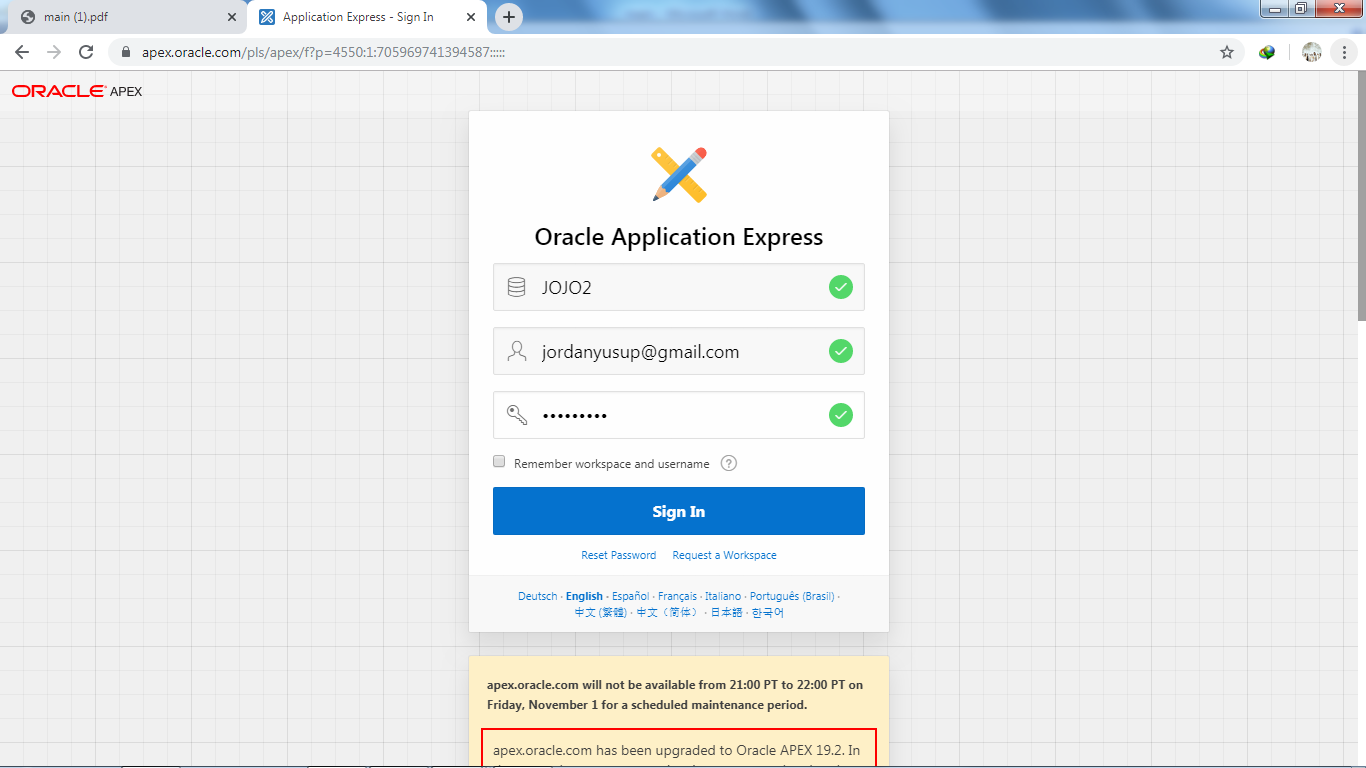
\includegraphics[width=12cm]{figures/Screenshot_2.png}
	\caption{Create Application}
\end{figure}
\item Oracle menyediakan banyak pilihan. Disini saya mencoba menggunakan “Movies”. Pilih Copy and Paste dan dari kotak "-Select Sample-" pilih "Movies" lalu klik "Next"
\begin{figure}[!htpb]
	\centering
	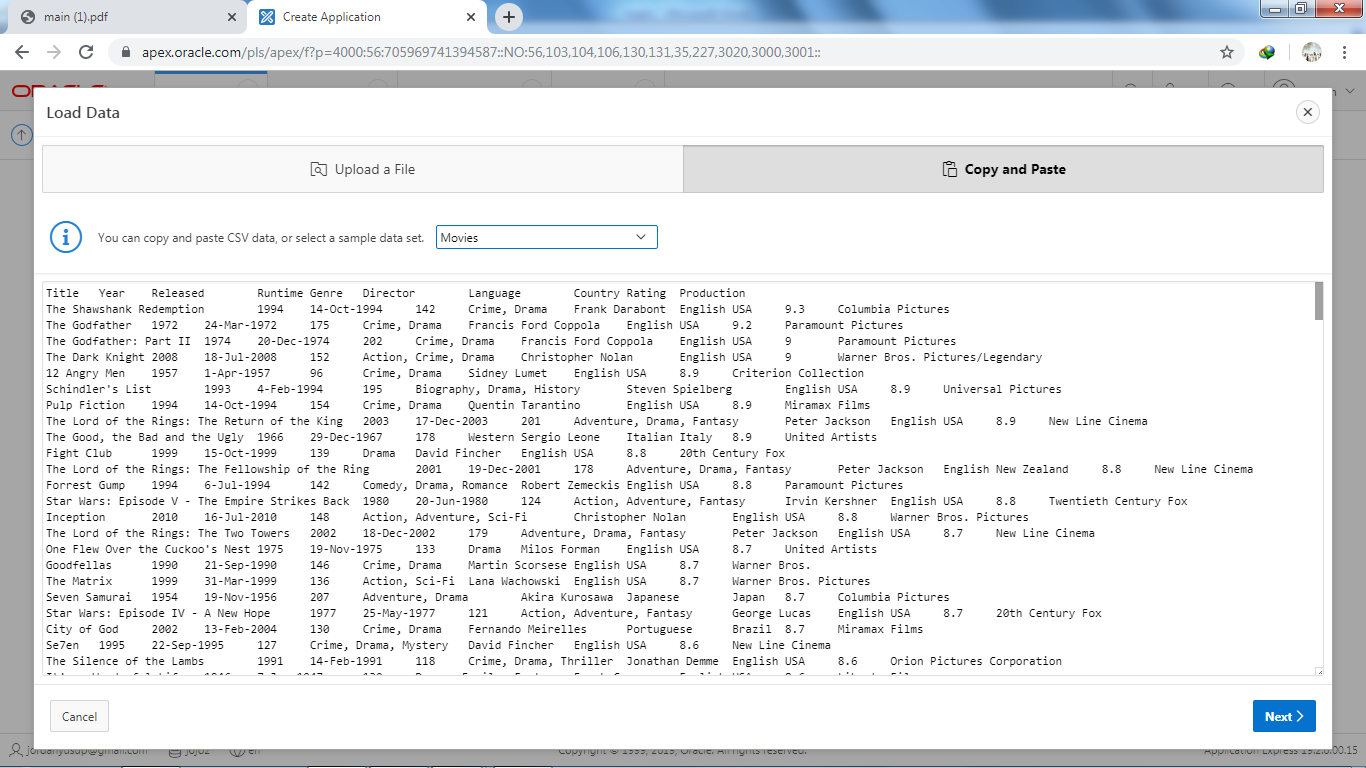
\includegraphics[width=12cm]{figures/Screenshot_3.png}
	\caption{Create Application}
\end{figure}
\item Agar tidak bingung Masukkan tabel name dengan nama MOVIES lalu klik Load Data dan tunggu sampai proses selesai.
\begin{figure}[!htpb]
	\centering
	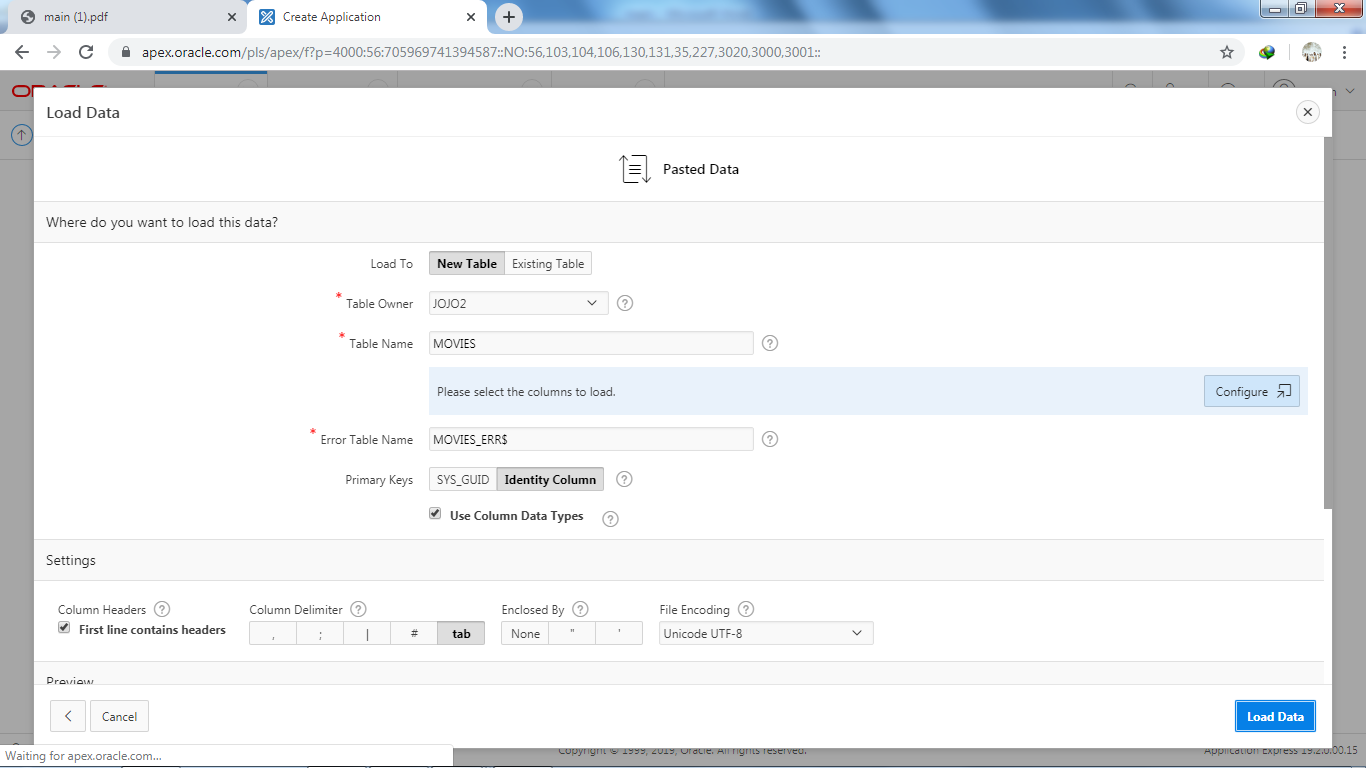
\includegraphics[width=12cm]{figures/Screenshot_4.png}
	\caption{Create Application}
\end{figure}
\item Lalu klik Create Application
\begin{figure}[!htpb]
	\centering
	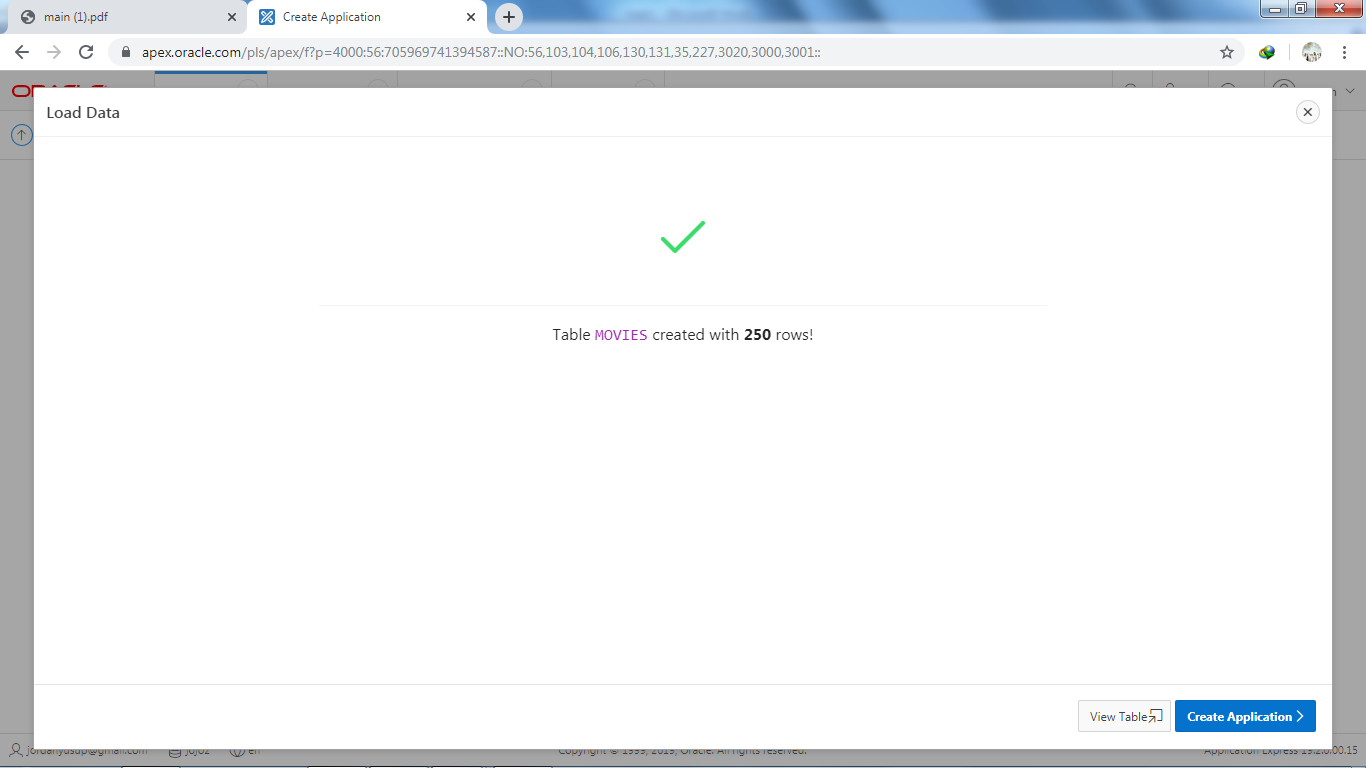
\includegraphics[width=12cm]{figures/Screenshot_5.png}
	\caption{Create Application}
\end{figure}
\item Scroll ke bawah dan pilih "Check all" di semua pilihan yang tersedia lalu Klik "Create Application". Tunggu proses sampai selesai.
\begin{figure}[!htpb]
	\centering
	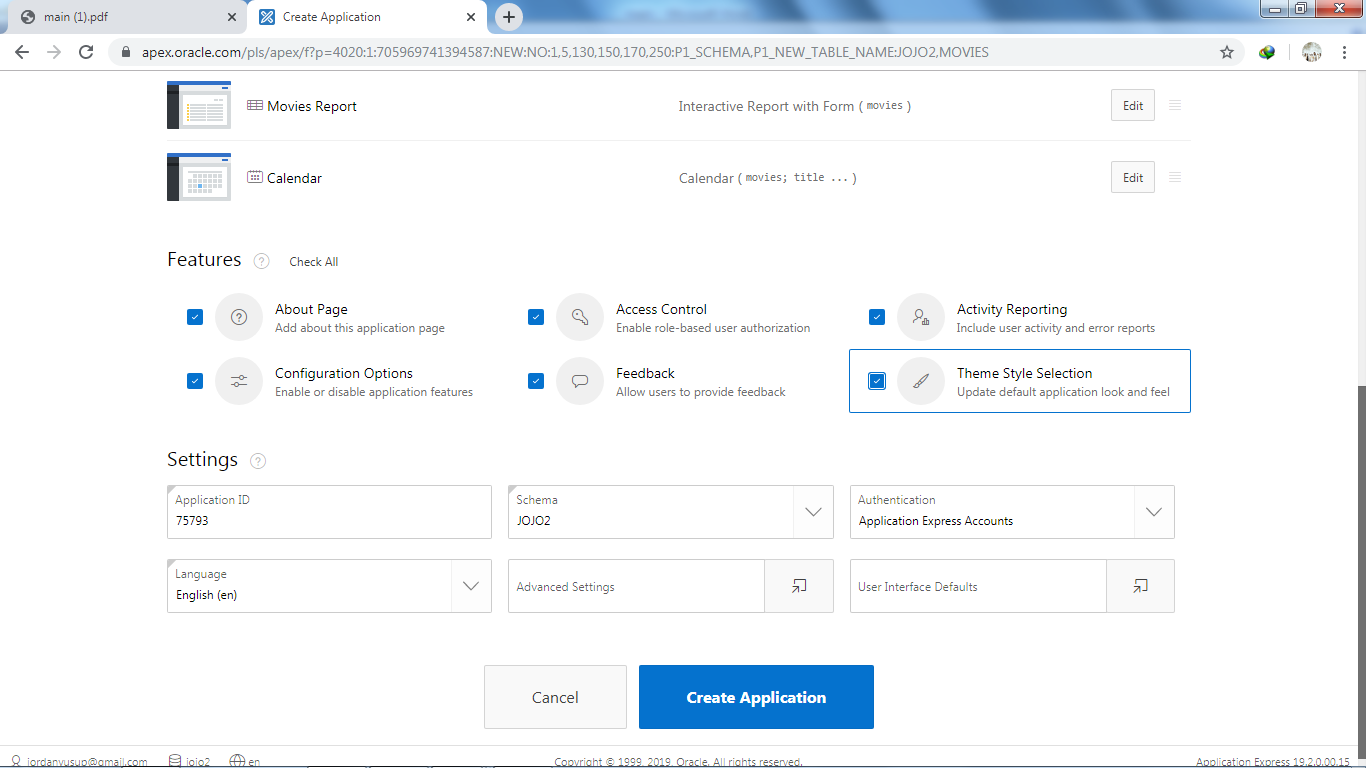
\includegraphics[width=12cm]{figures/Screenshot_6.png}
	\caption{Create Application}
\end{figure}
\item Taraa Aplikasi telah selesai dan siap dijalankan klik "Run Application".
\begin{figure}[!htpb]
	\centering
	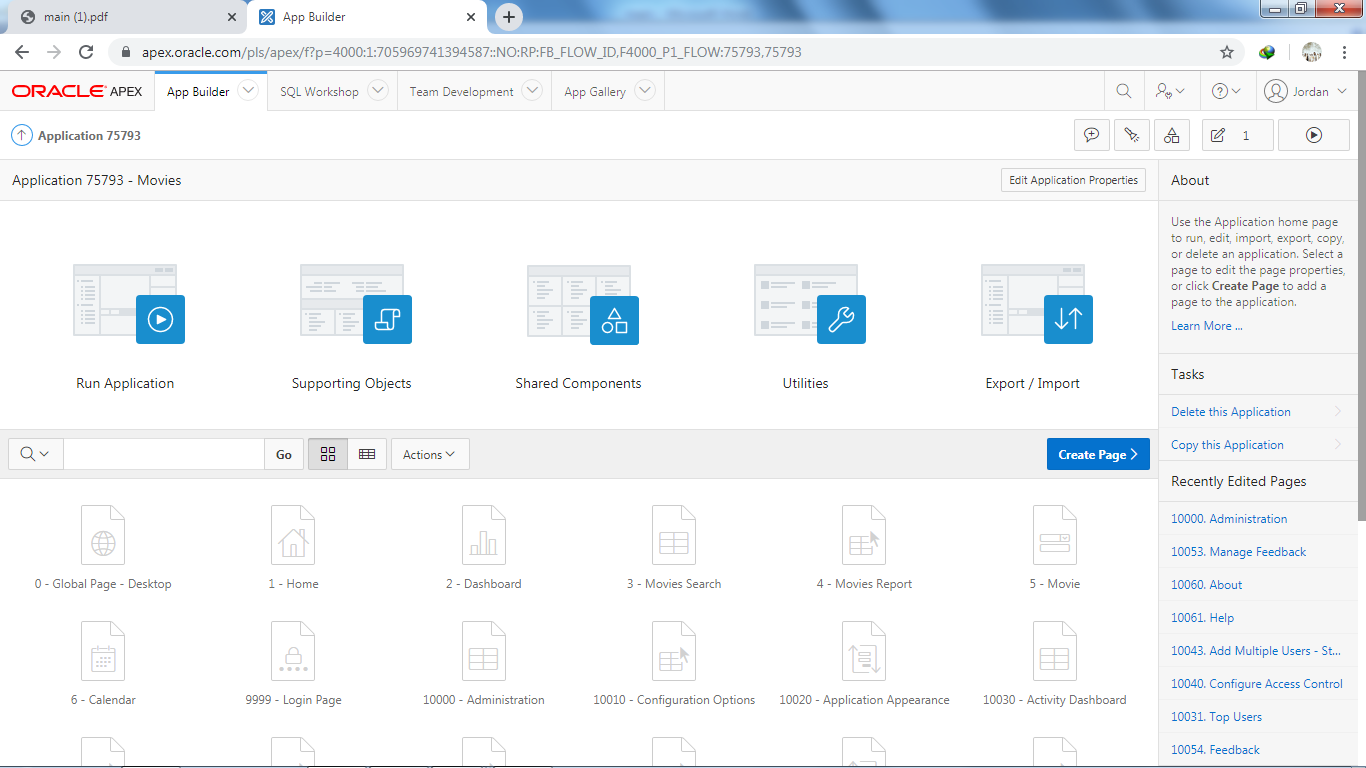
\includegraphics[width=12cm]{figures/Screenshot_7.png}
	\caption{Create Application}
\end{figure}
\item Silahkan login untuk masuk ke aplikasi yang telah kita buat tadi.
\begin{figure}[!htpb]
	\centering
	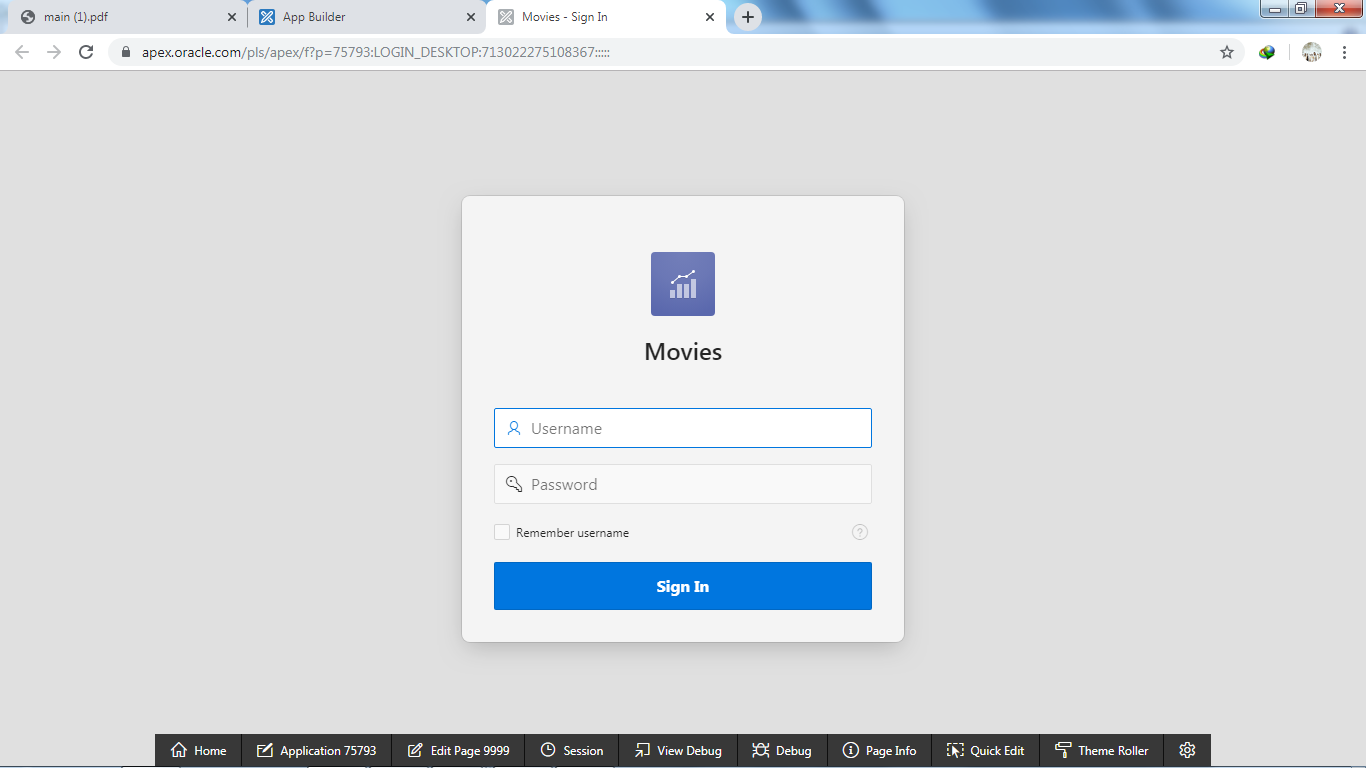
\includegraphics[width=12cm]{figures/Screenshot_8.png}
	\caption{Movies Application}
\end{figure}
\item Tampilan Utama dari Movies Application yang kita buat, silahkan klik dan amati menu-menu dari aplikasi ini.
\begin{figure}[!htpb]
	\centering
	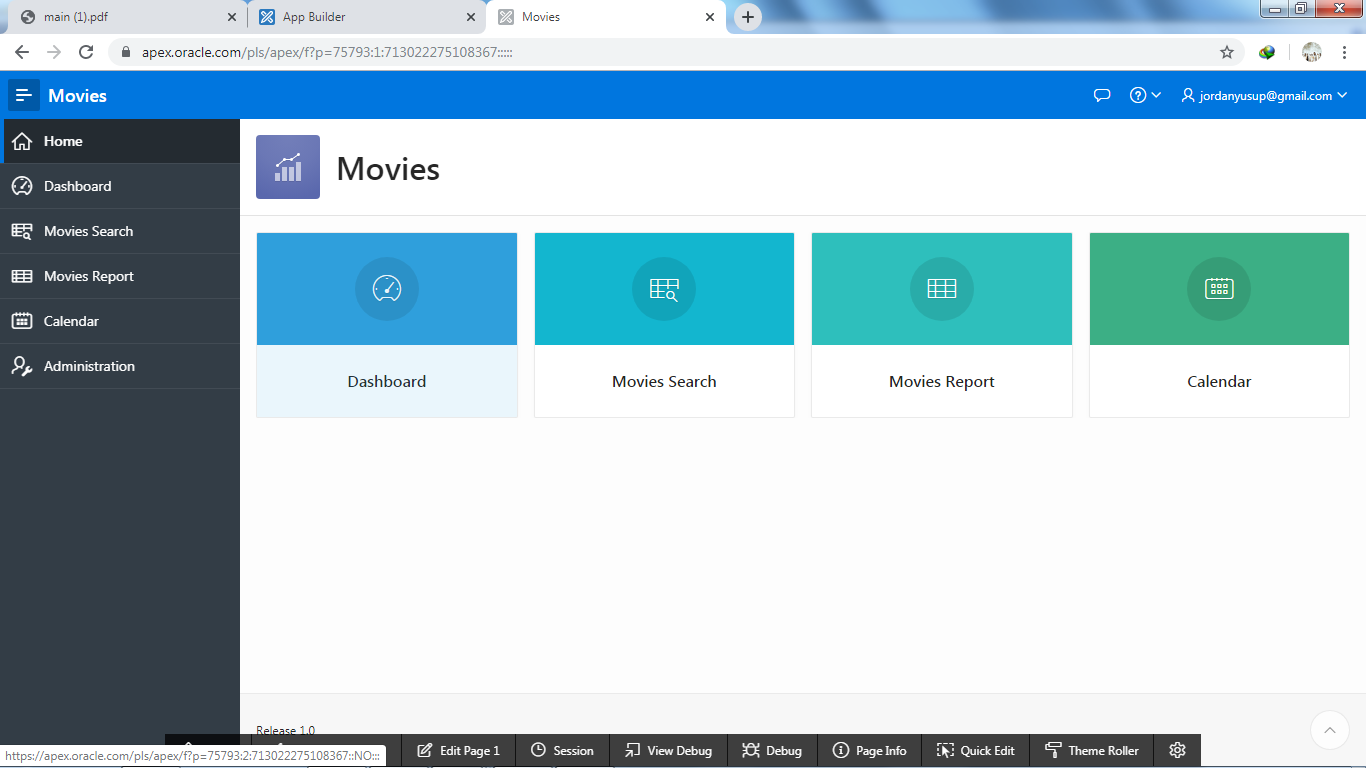
\includegraphics[width=12cm]{figures/Screenshot_9.png}
	\caption{Movies Application}
\end{figure}
\item Sekarang Mari kita coba mengecek table yang ada didalam movies dengan mengetik sintaks "Select * from movies" di SQL Commands.
\begin{figure}[!htpb]
	\centering
	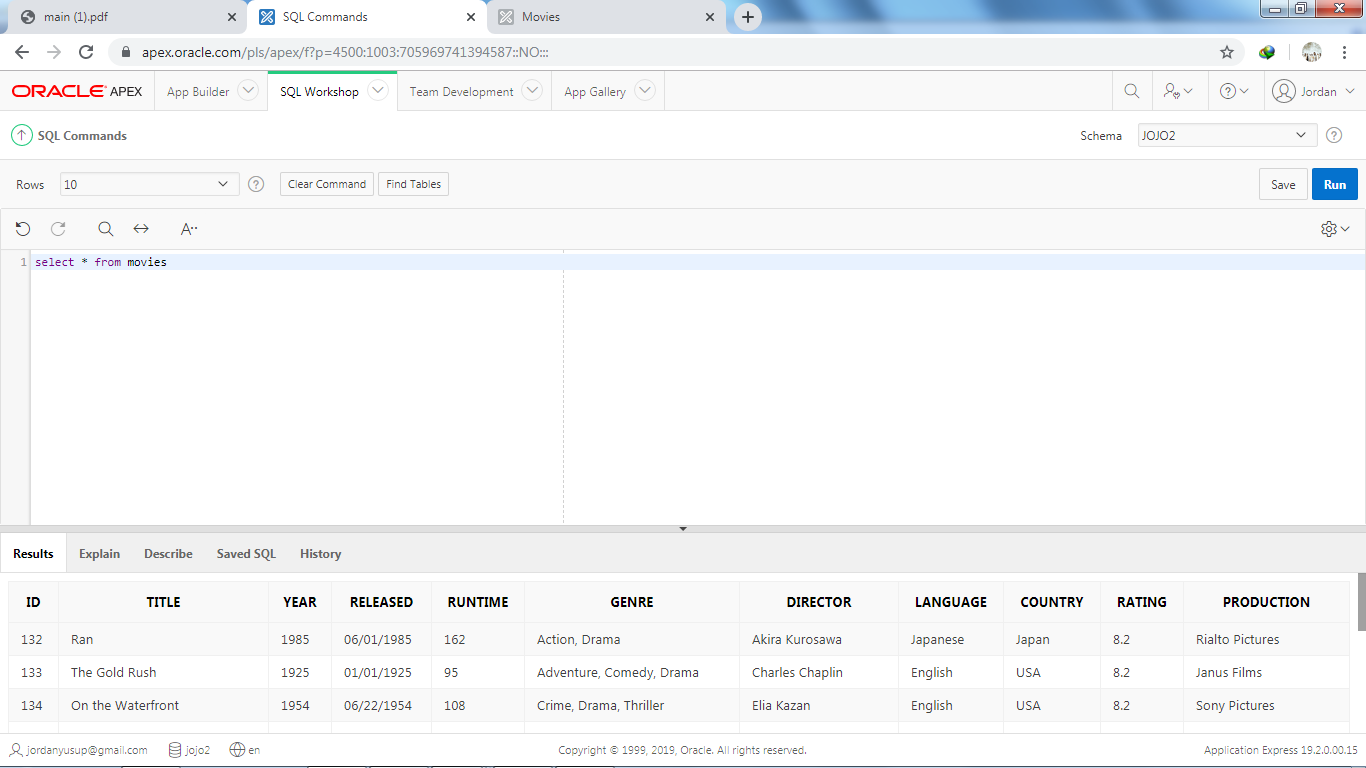
\includegraphics[width=12cm]{figures/Screenshot_10.png}
	\caption{Movies Application}
\end{figure}
\end{itemize}
\section{Quick SQL}
Quick SQL adalah bahasa yang dapat membantu Kita untuk menghasilkan kode SQL yang benar secara sistematis untuk mendesain database dan diimplementasikan dengan cepat dari membuat tabeln untuk membuat aplikasi database dan semua tabel itu dapat di Generate.\\
\subsection{Cara Menggunakan Quick SQL}
\begin{itemize}
\item Di Halaman Utama apex oracle, klik tab "SQL Workshop" lalu Pilih "Utilities" kemudian Pilih "Quick SQL" setelah itu akan muncul tampilan seperti di bawah.
\begin{figure}[!htpb]
	\centering
	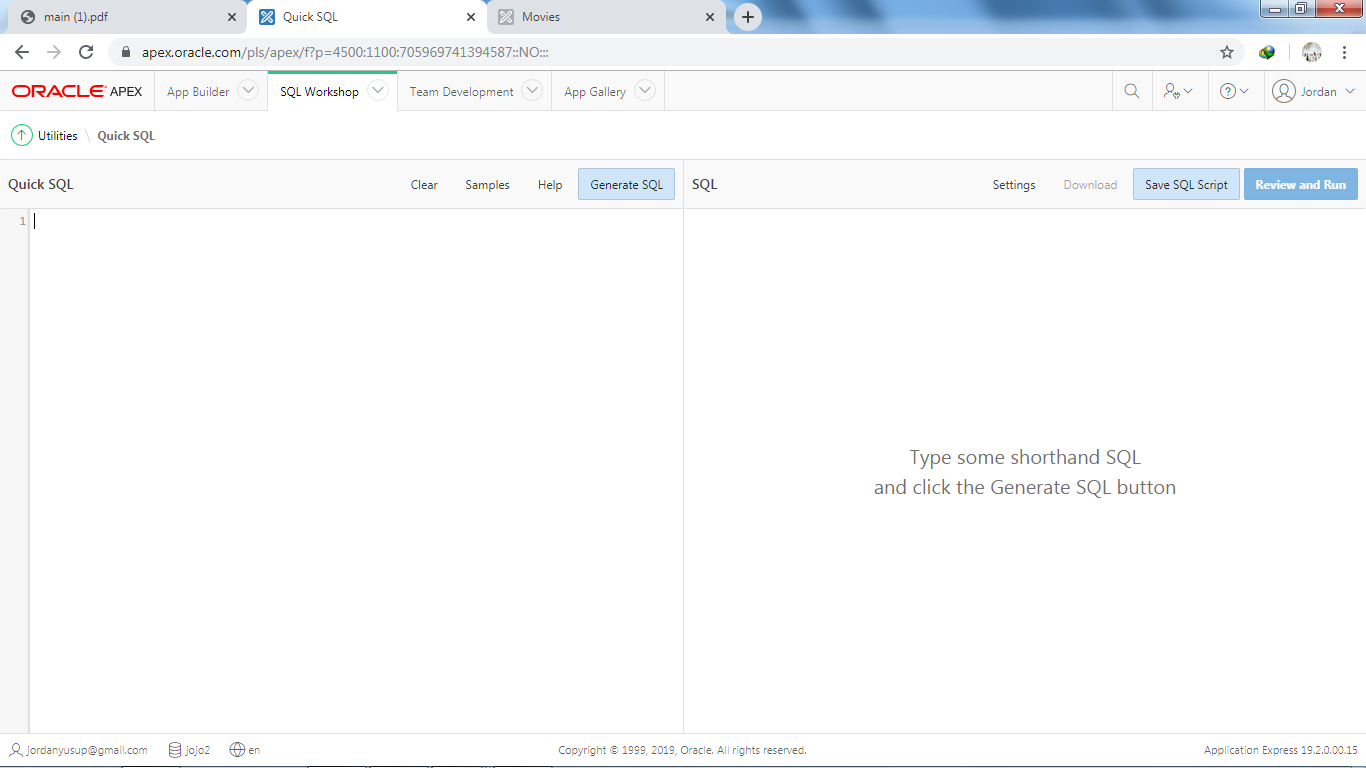
\includegraphics[width=10cm]{figures/Screenshot_11.png}
	\caption{Quick SQL}
\end{figure}
\item Di halaman quick sql kita pilih "samples" sebagai contoh , lalu akan muncul tampilan di bawah dan pilih "Load data" pada "Employees Skills". Disini saya mencoba menggunakan employees skilss
\begin{figure}[!htpb]
	\centering
	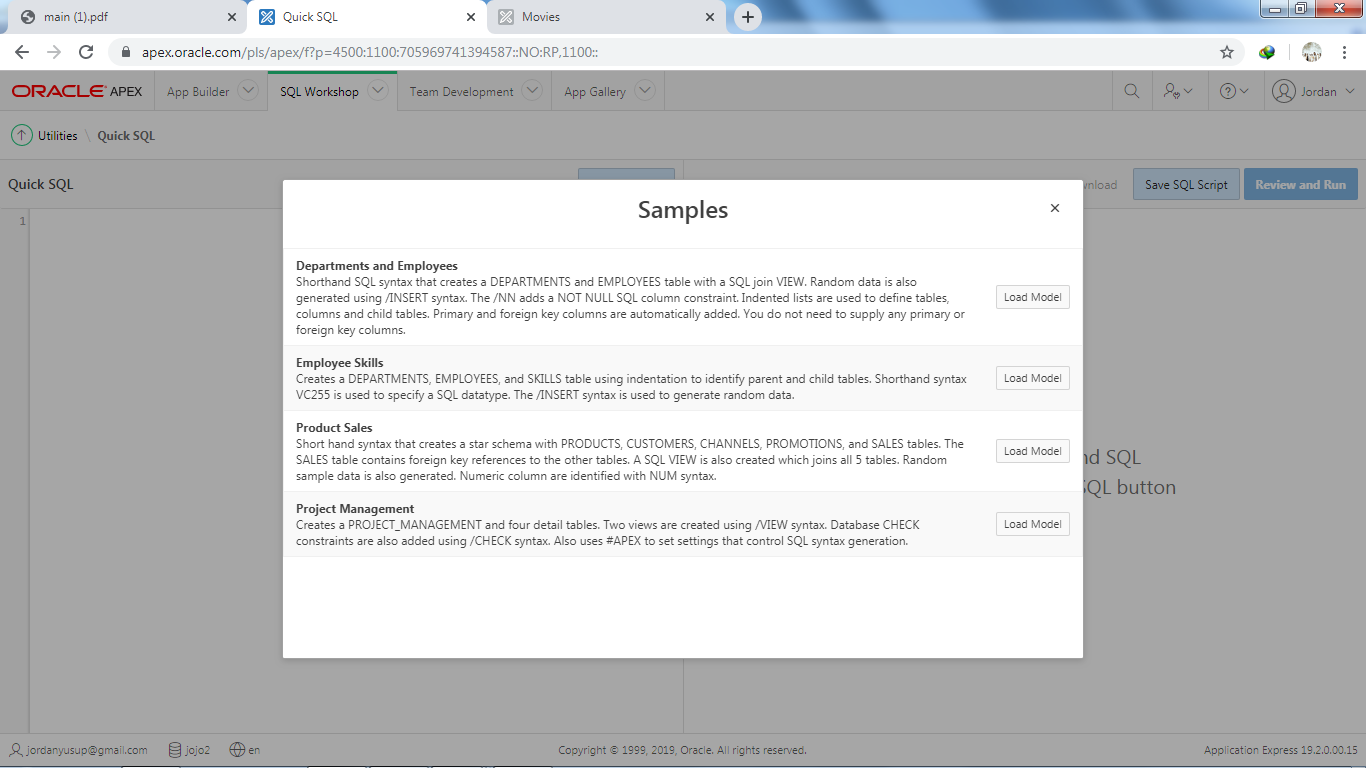
\includegraphics[width=11cm]{figures/Screenshot_12.png}
	\caption{Quick SQL}
\end{figure}
\item Setelah di Load Data akan muncul sintaks dari employees skill yang kita coba tadi seperti di bawah.
\begin{figure}[!htpb]
	\centering
	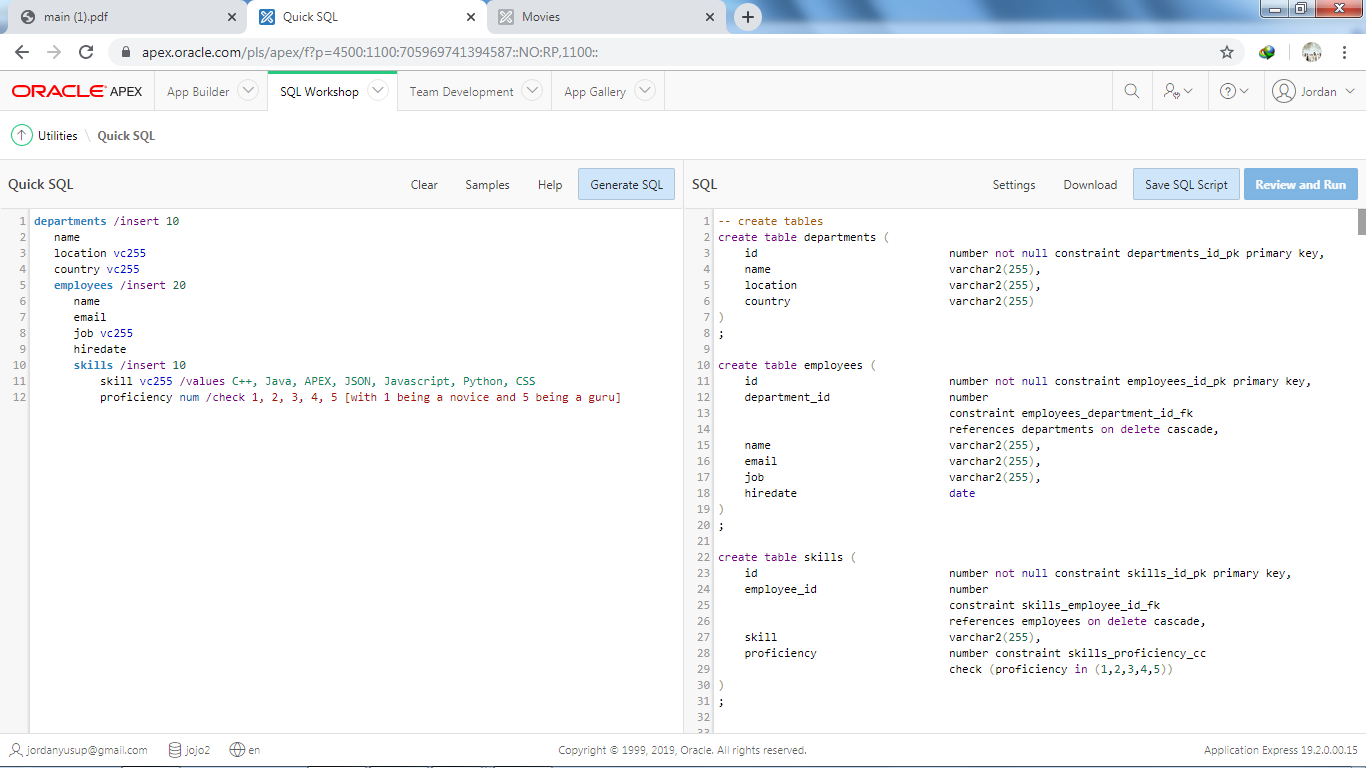
\includegraphics[width=12.5cm]{figures/Screenshot_13.png}
	\caption{Quick SQL}
\end{figure}
\item Pergi ke settings, lalu muncul konfigurasi seperti di bawah. Kita mencoba menambahkan kata apac pada sintaks diatas
\begin{figure}[!htpb]
	\centering
	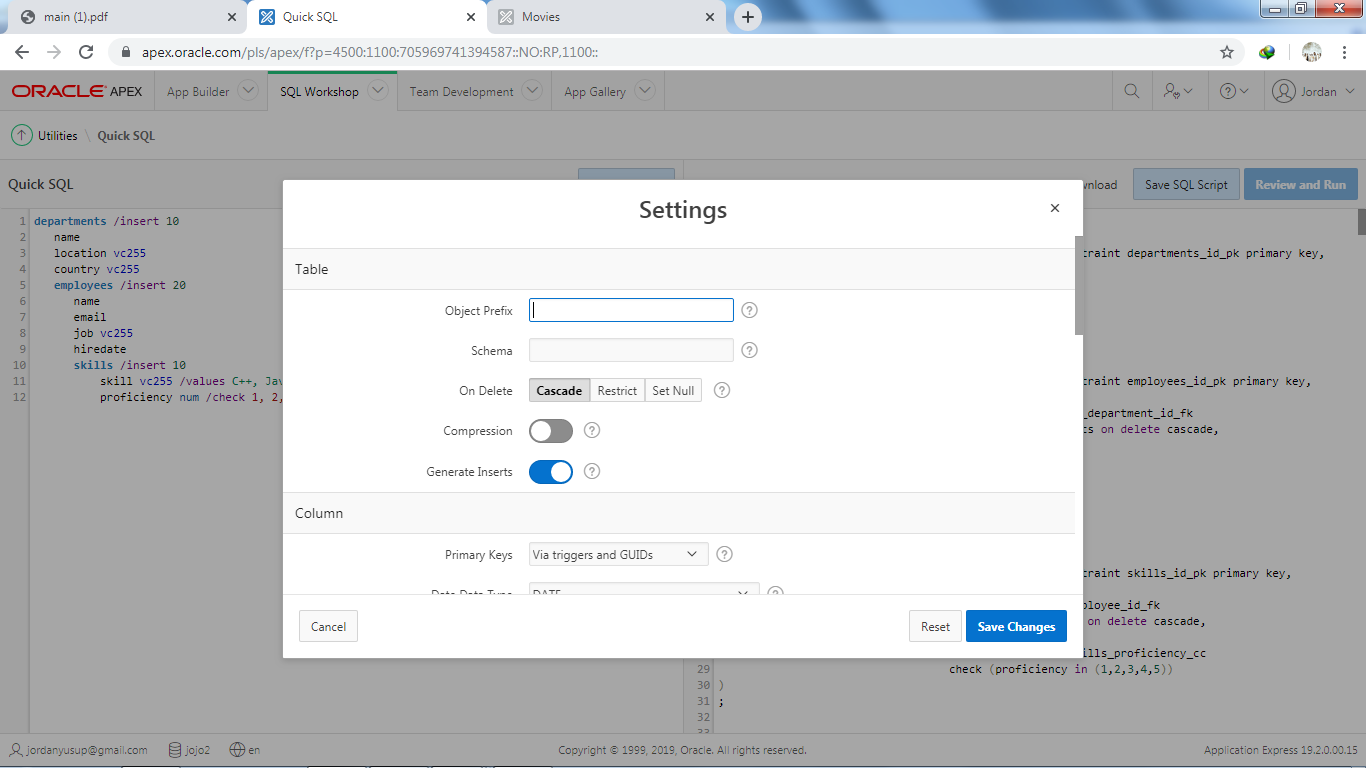
\includegraphics[width=12.5cm]{figures/Screenshot_14.png}
	\caption{Quick SQL}
\end{figure}
\item Scroll ke bawah, cari "Include Drops" lalu centang dan save.
\begin{figure}[!htpb]
	\centering
	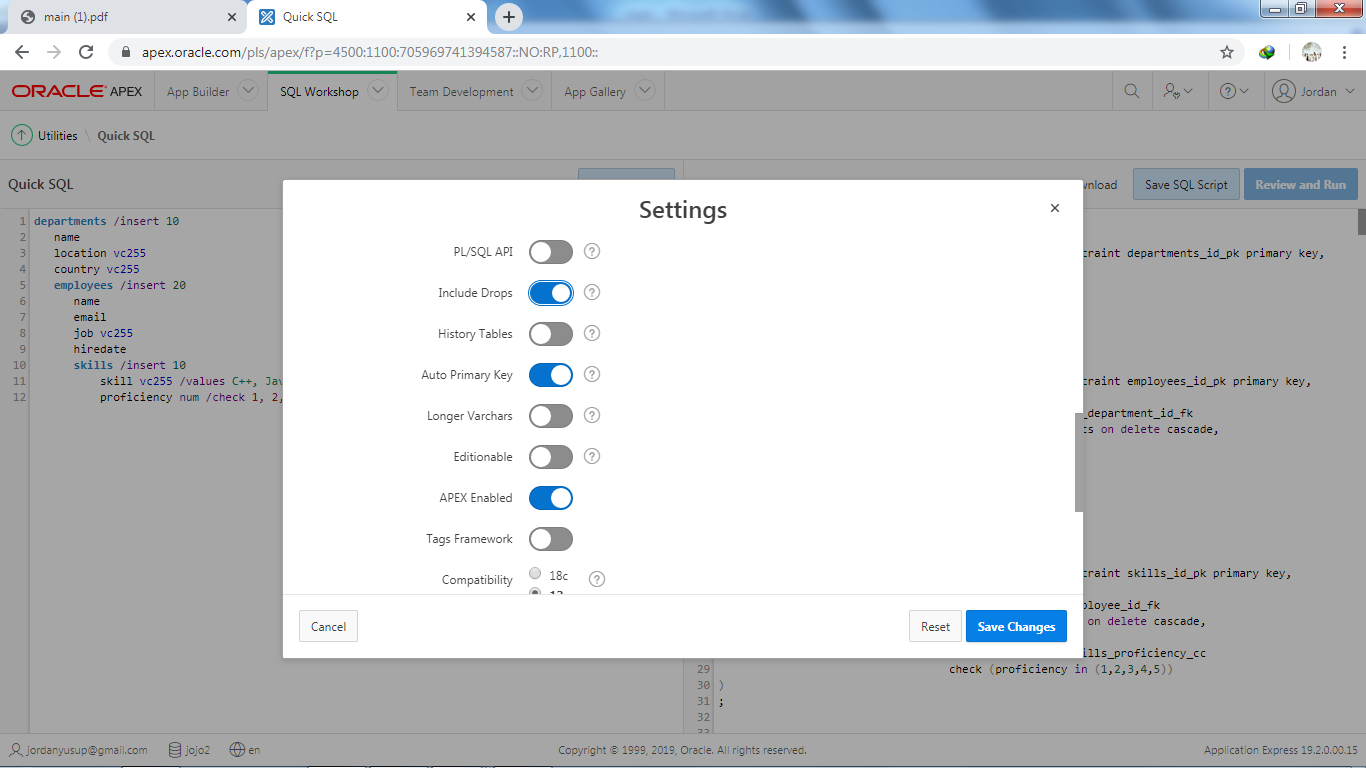
\includegraphics[width=12.5cm]{figures/Screenshot_15.png}
	\caption{Quick SQL}
\end{figure}
\item Setelah itu akan ada perubahan pada tab SQL,akan ada penambahan kata apac dan bisa di lihat di bawah.
\begin{figure}[!htpb]
	\centering
	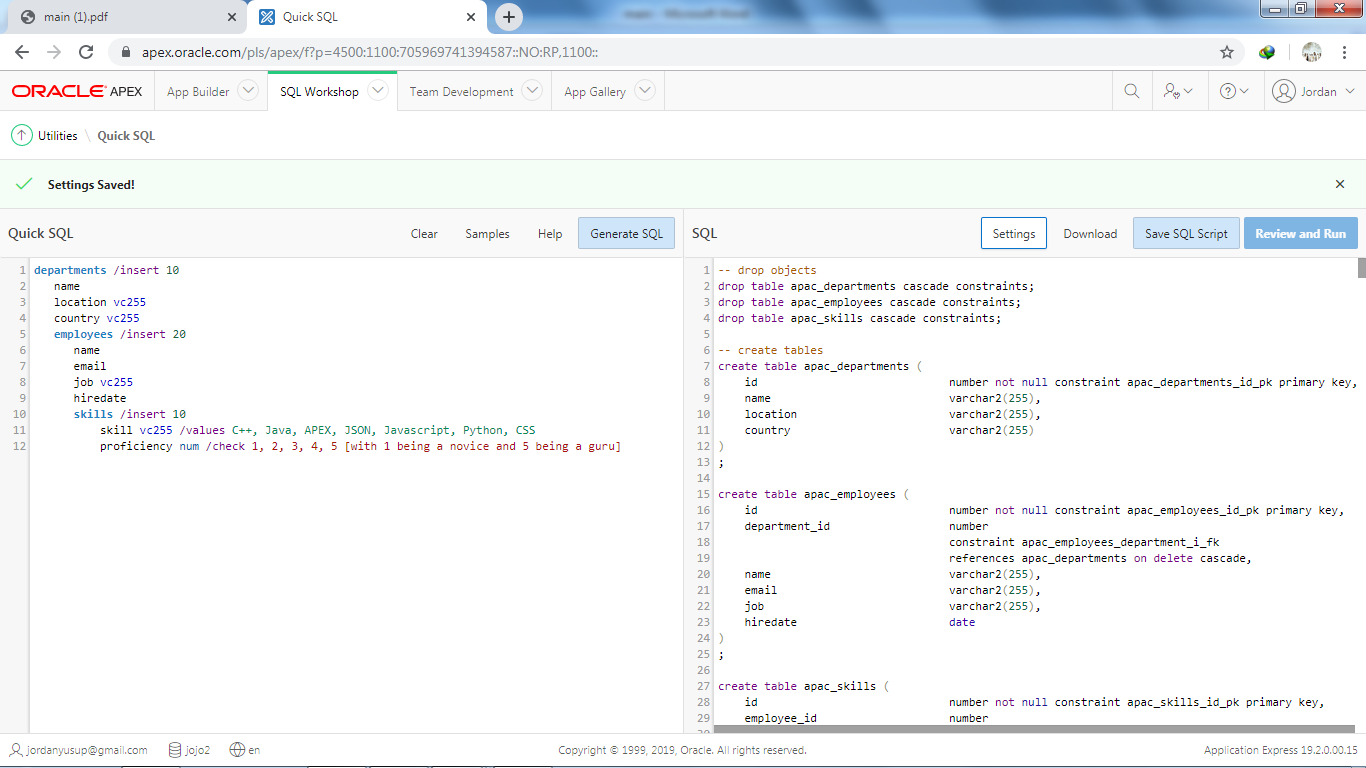
\includegraphics[width=12.5cm]{figures/Screenshot_16.png}
	\caption{Quick SQL}
\end{figure}
\item Klik "Save SQL Script" dan beri nama apac karena tadi kita menambahkan kata apac.
\begin{figure}[!htpb]
	\centering
	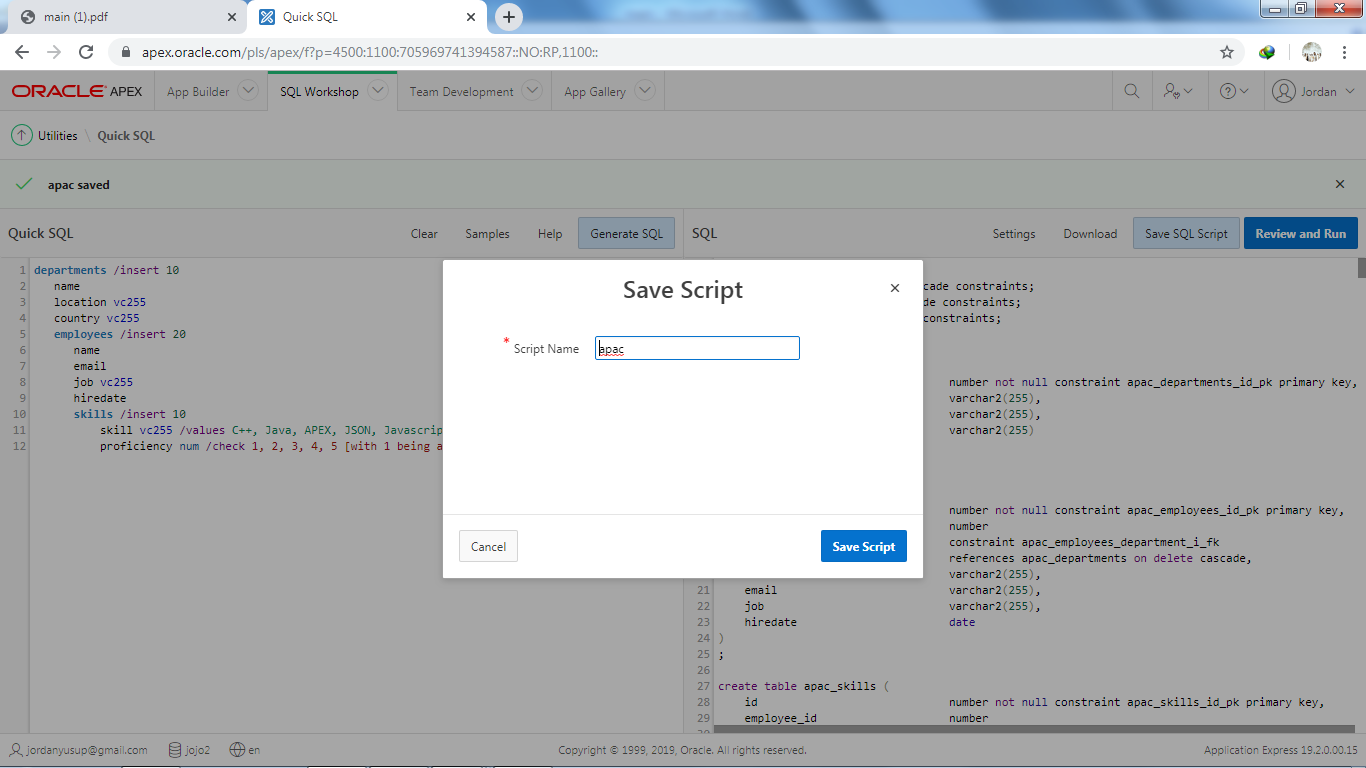
\includegraphics[width=12.5cm]{figures/Screenshot_17.png}
	\caption{Quick SQL}
\end{figure}
\item Lalu Klik "Review and Run" dan akan muncul tampilan seperti di bawah dan klik "Save" untuk menjalankan sintaks tadi.
\begin{figure}[!htpb]
	\centering
	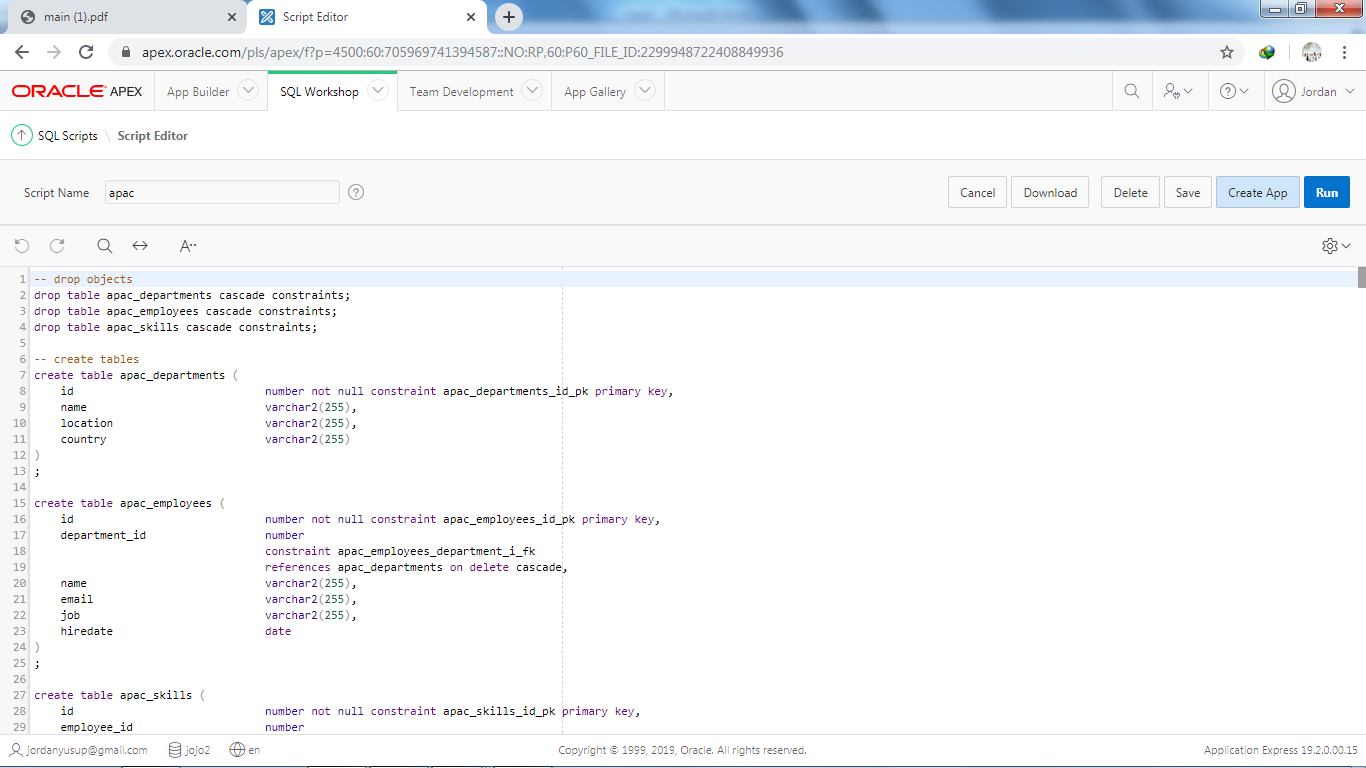
\includegraphics[width=12.5cm]{figures/Screenshot_18.png}
	\caption{Quick SQL}
\end{figure}
\item Klik "Run" pada script apac yang dibuat tadi.
\begin{figure}[!htpb]
	\centering
	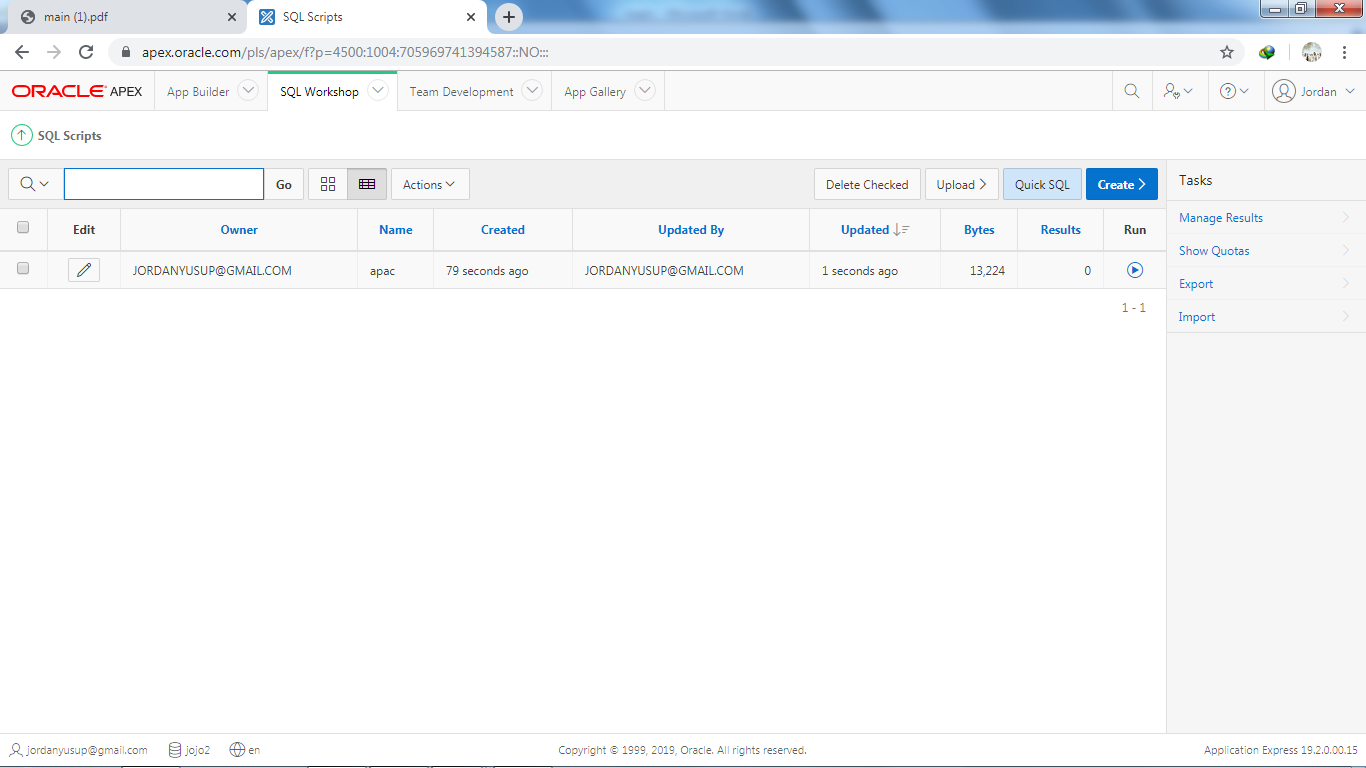
\includegraphics[width=12cm]{figures/Screenshot_19.png}
	\caption{Quick SQL}
\end{figure}
\item Lalu akan muncul halaman Run Script, Klik "Run Now".
\begin{figure}[!htpb]
	\centering
	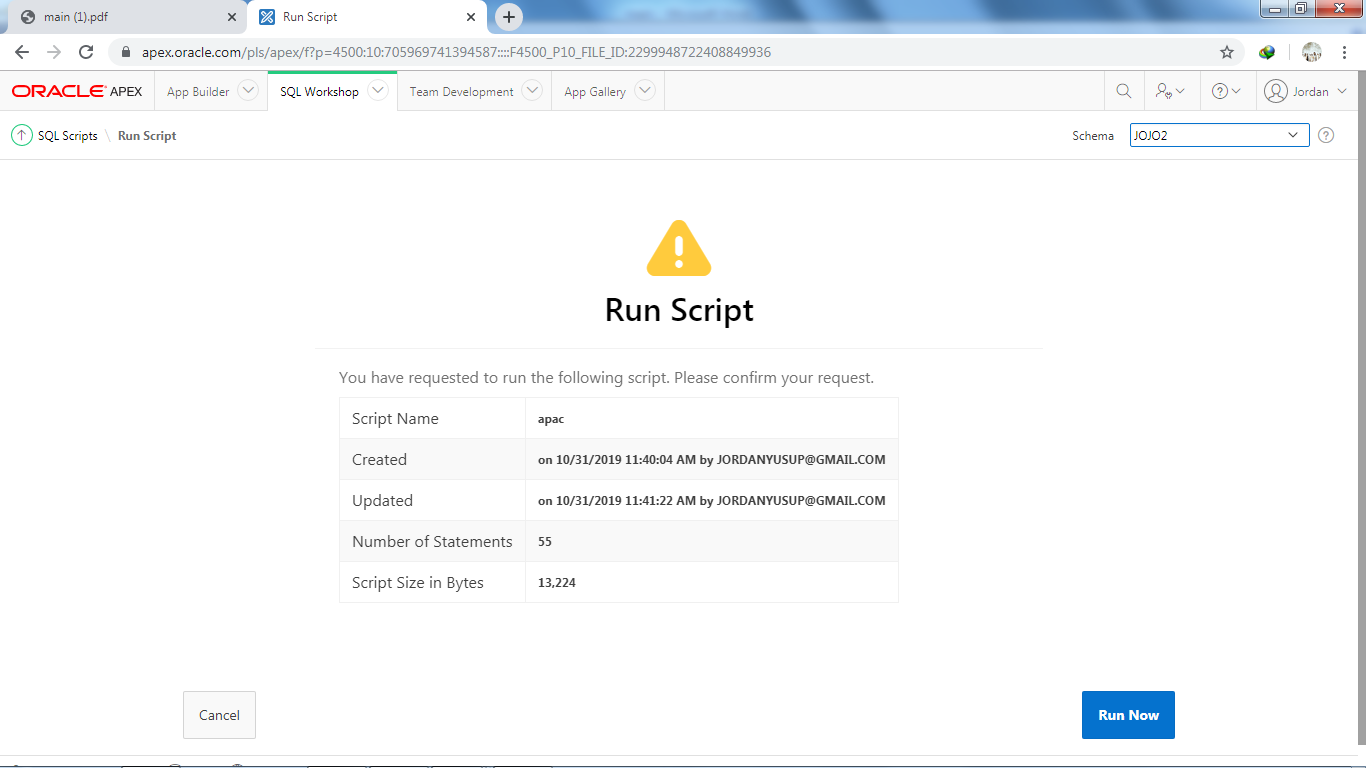
\includegraphics[width=12cm]{figures/Screenshot_20.png}
	\caption{Quick SQL}
\end{figure}
\item Akan muncul halaman Results, dimana menampilkan detail dari aplikasi yang akan dibuat.
\begin{figure}[!htpb]
	\centering
	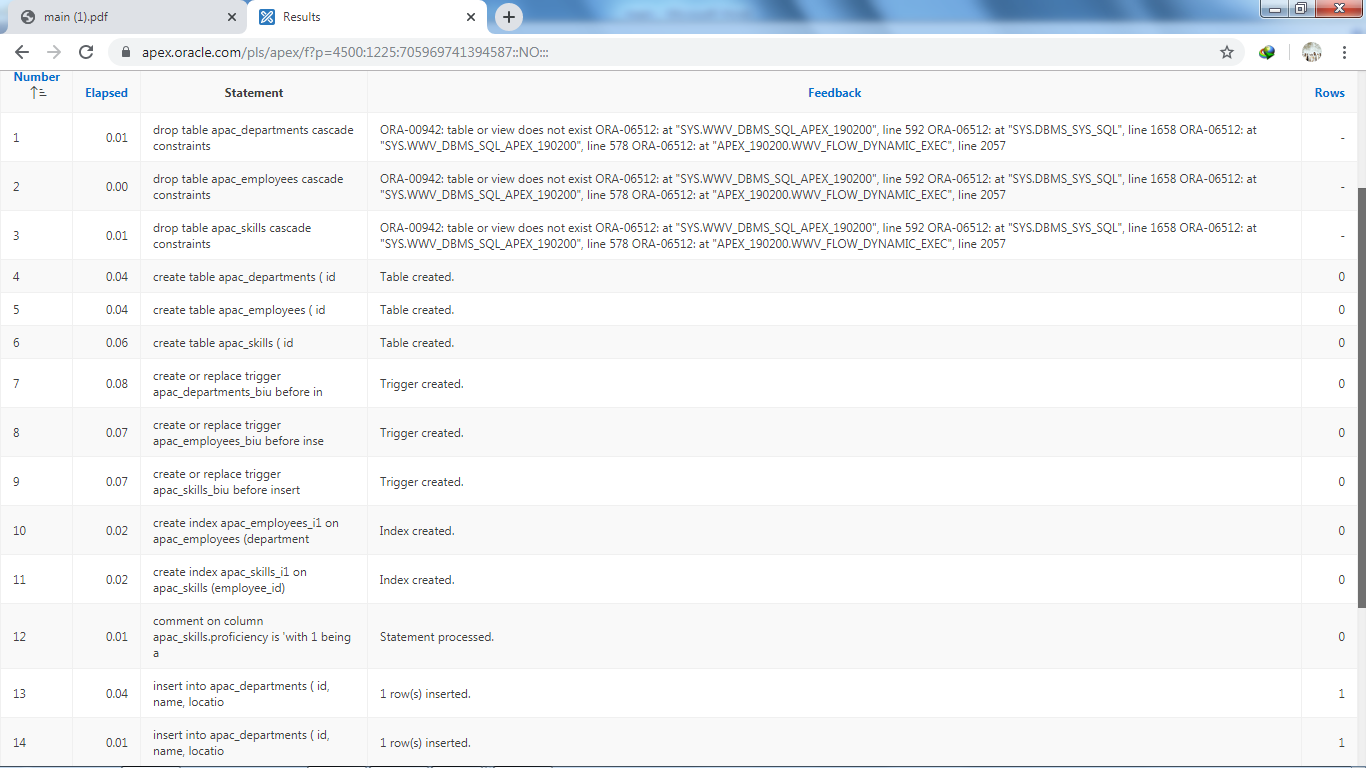
\includegraphics[width=12cm]{figures/Screenshot_21.png}
	\caption{Quick SQL}
\end{figure}
\item Lalu tekan "Create App" dan pilih "Create Application".
\begin{figure}[!htpb]
	\centering
	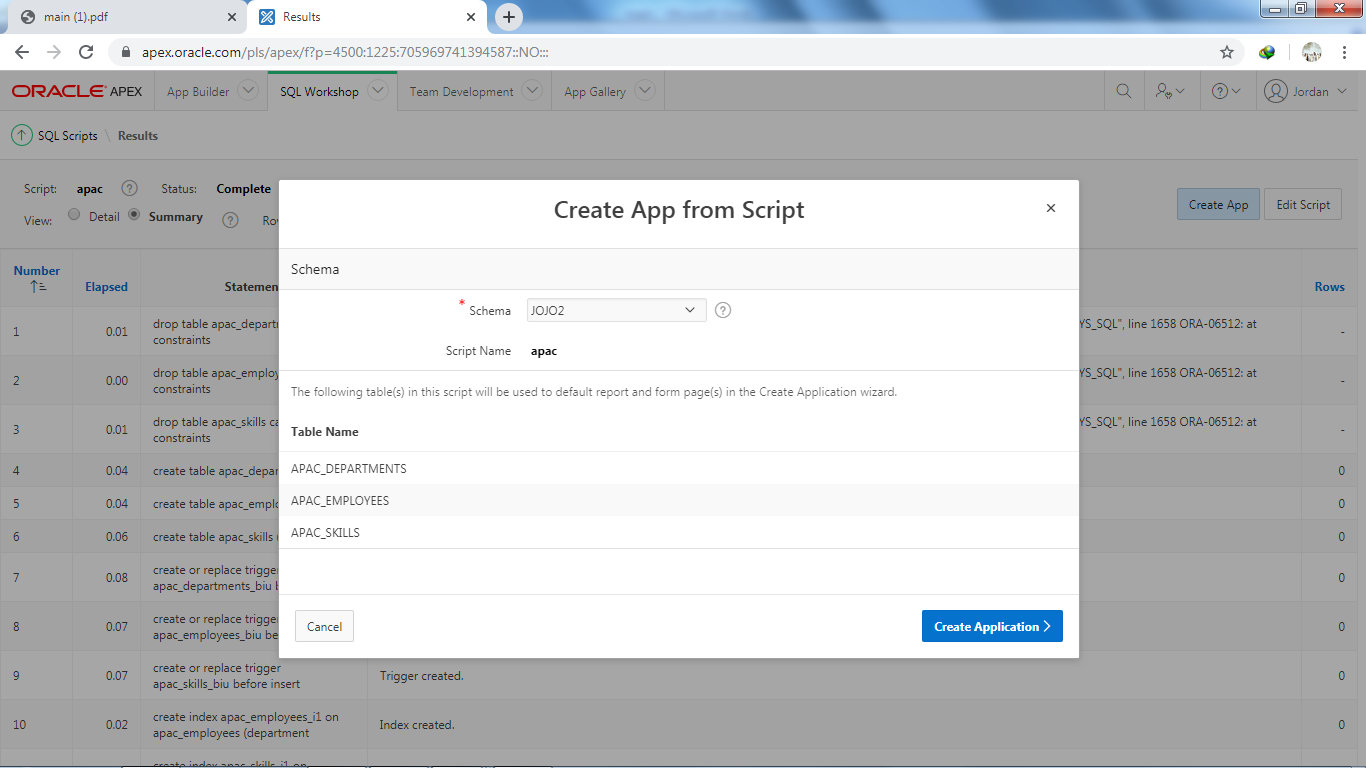
\includegraphics[width=12cm]{figures/Screenshot_22.png}
	\caption{Quick SQL}
\end{figure}
\item Jika telah dibuat silahkan Run Application lalu Login dan terakhir halaman aplikasinya akan muncul dan selesai membuat aplikasi.
\begin{figure}[!htpb]
	\centering
	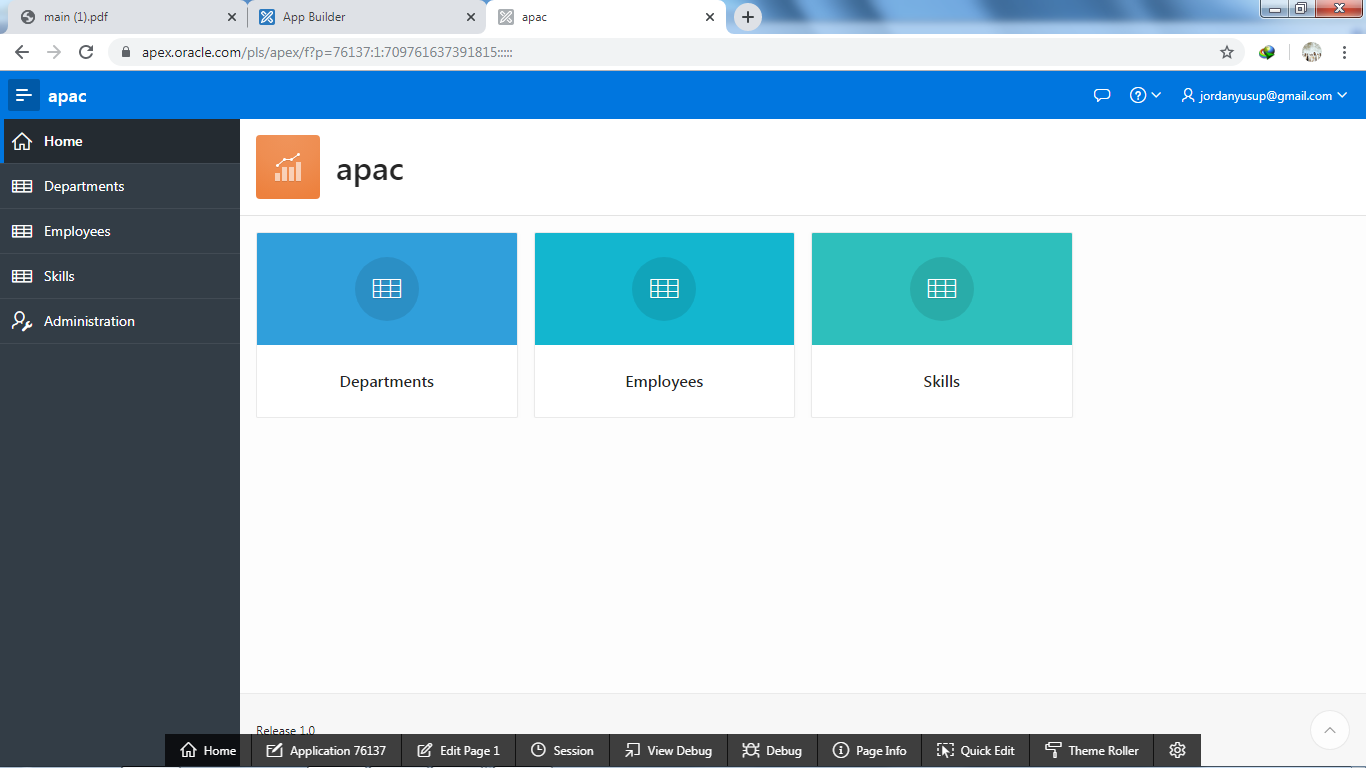
\includegraphics[width=12cm]{figures/Screenshot_23.png}
	\caption{Quick SQL}
\end{figure}
\end{itemize}
\section{Membuat Aplikasi dari App Gallery}
Pada App Gallery terdapat beberapa aplikasi yang sudah tersedia dan untuk menggunakannya cukup lakukan instalasi saja. Berikut cara instalasi aplikasi "Sample Charts".

\begin{itemize}
\item Seperti pada biasanya login ke apex.oracle, jika sudah klik "App Gallery".
\begin{figure}[!htpb]
	\centering
	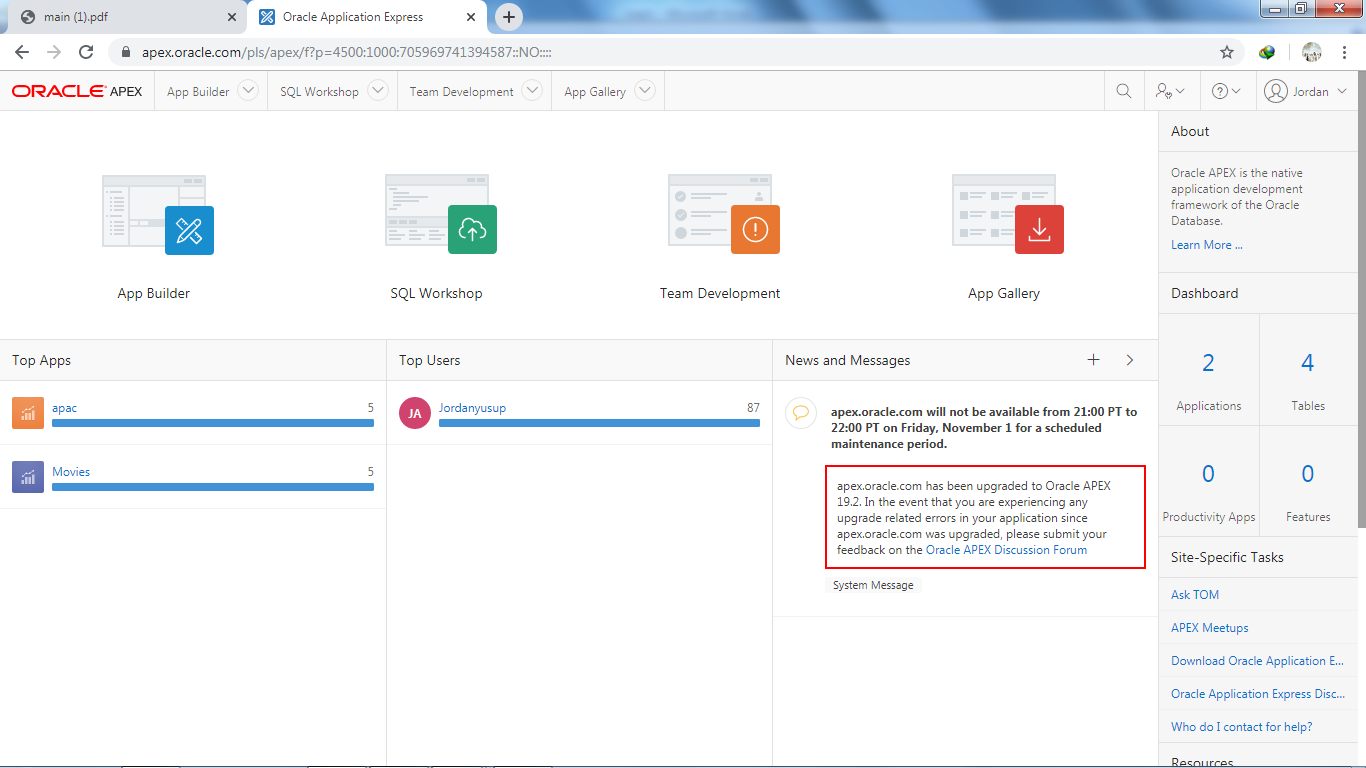
\includegraphics[width=12cm]{figures/Screenshot_24.png}
	\caption{App Gallery}
\end{figure}
\item Akan muncul halaman App Gallery dan pilih "Sample".
\begin{figure}[!htpb]
	\centering
	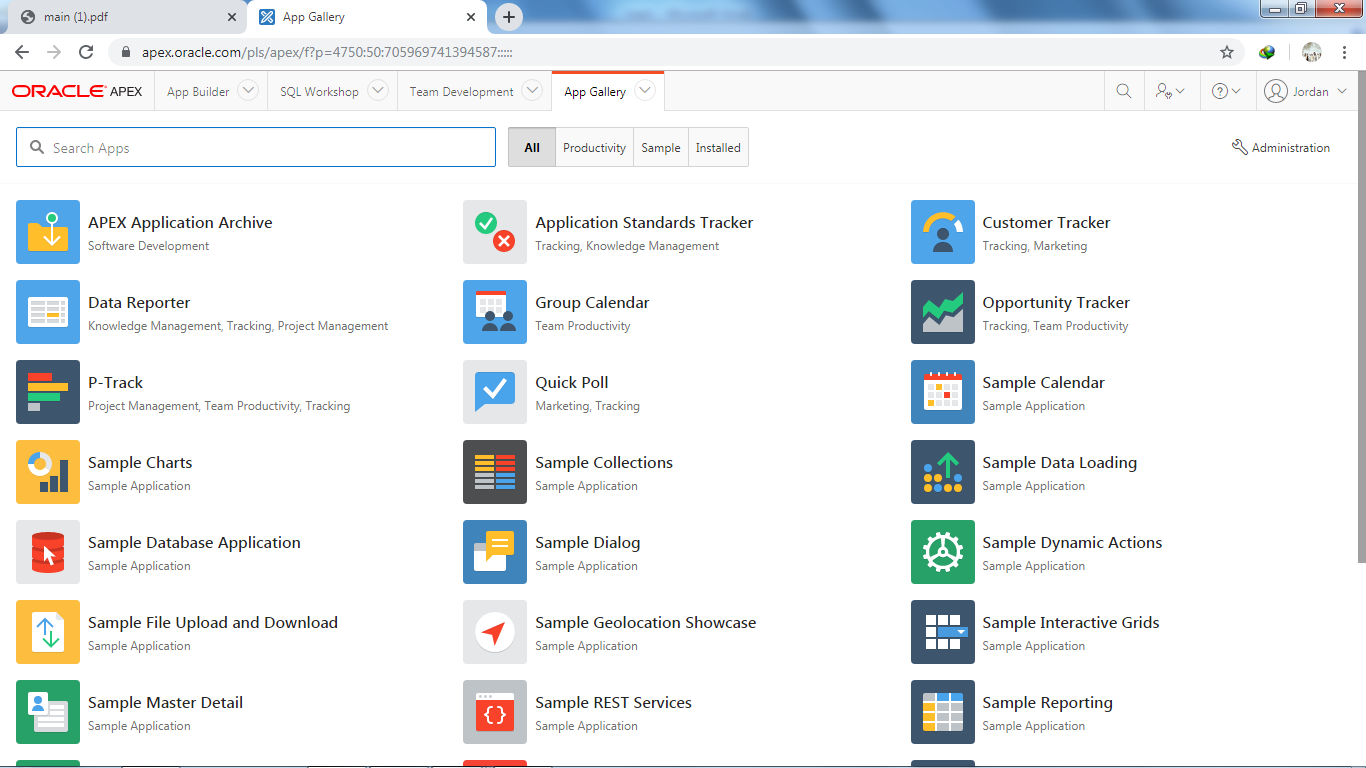
\includegraphics[width=12cm]{figures/Screenshot_25.png}
	\caption{App Gallery}
\end{figure}
\item Pilih "Sample Charts".
\begin{figure}[!htpb]
	\centering
	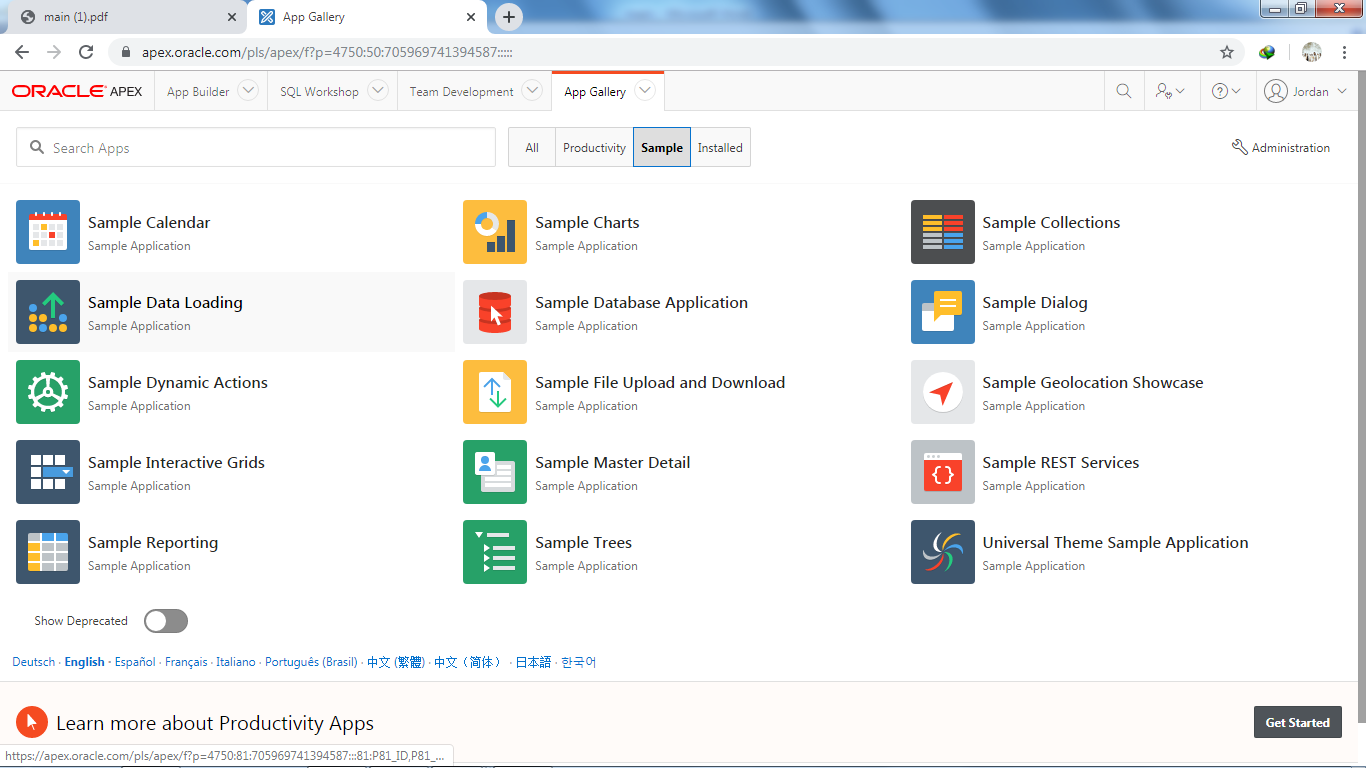
\includegraphics[width=12.5cm]{figures/Screenshot_26.png}
	\caption{App Gallery}
\end{figure}
\item Pilih "Install App".
\begin{figure}[!htpb]
	\centering
	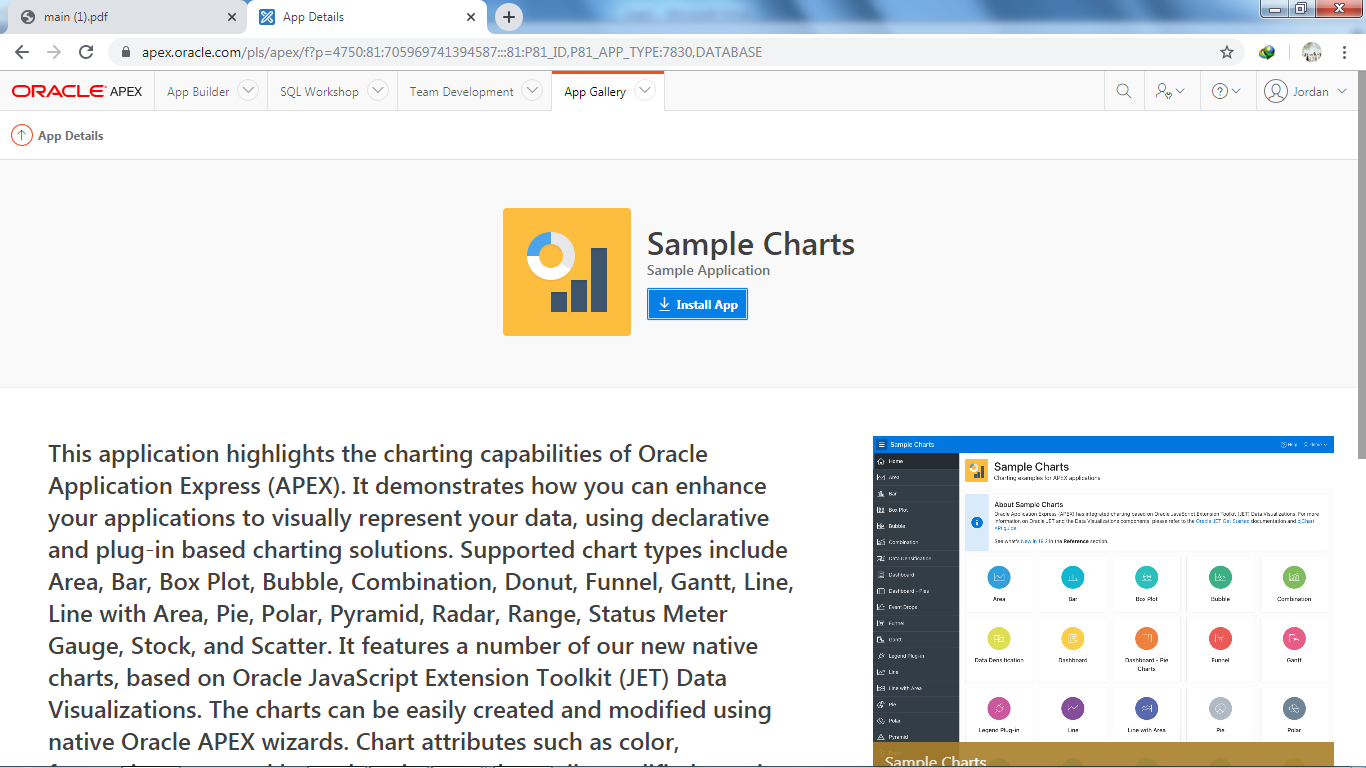
\includegraphics[width=12.5cm]{figures/Screenshot_27.png}
	\caption{App Gallery}
\end{figure}
\item Klik "Next".
\begin{figure}[!htpb]
	\centering
	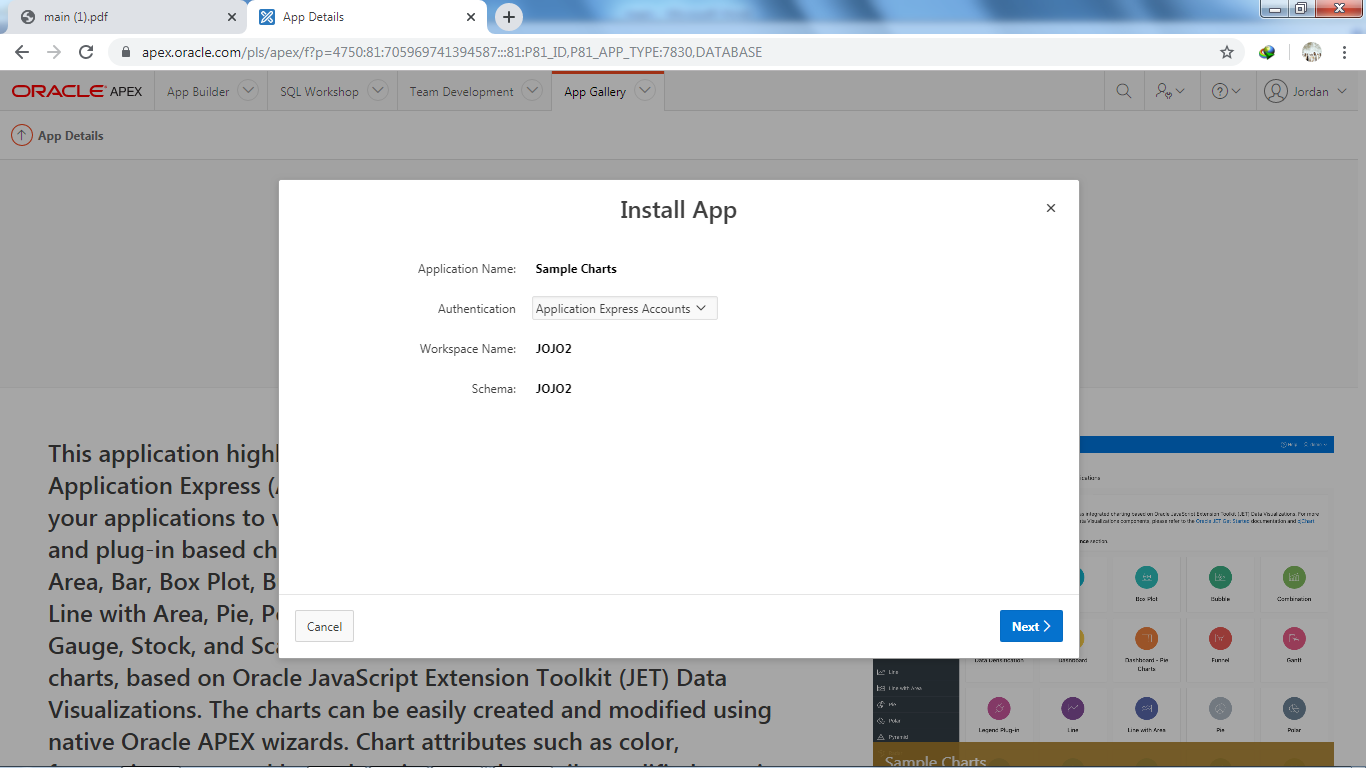
\includegraphics[width=12.5cm]{figures/Screenshot_28.png}
	\caption{App Gallery}
\end{figure}
\item Klik "Install App".
\begin{figure}[!htpb]
	\centering
	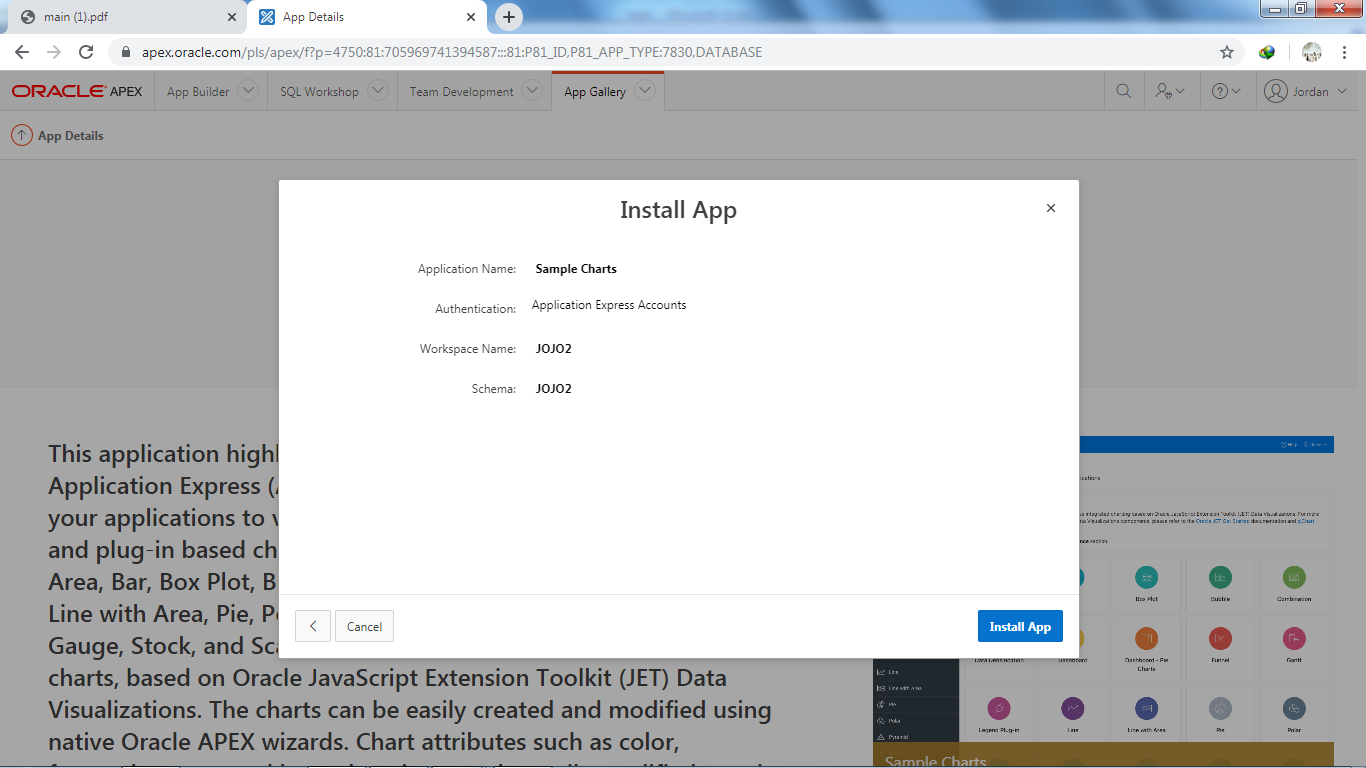
\includegraphics[width=12.5cm]{figures/Screenshot_29.png}
	\caption{App Gallery}
\end{figure}
\item Klik tombol "Run Application".
\begin{figure}[!htpb]
	\centering
	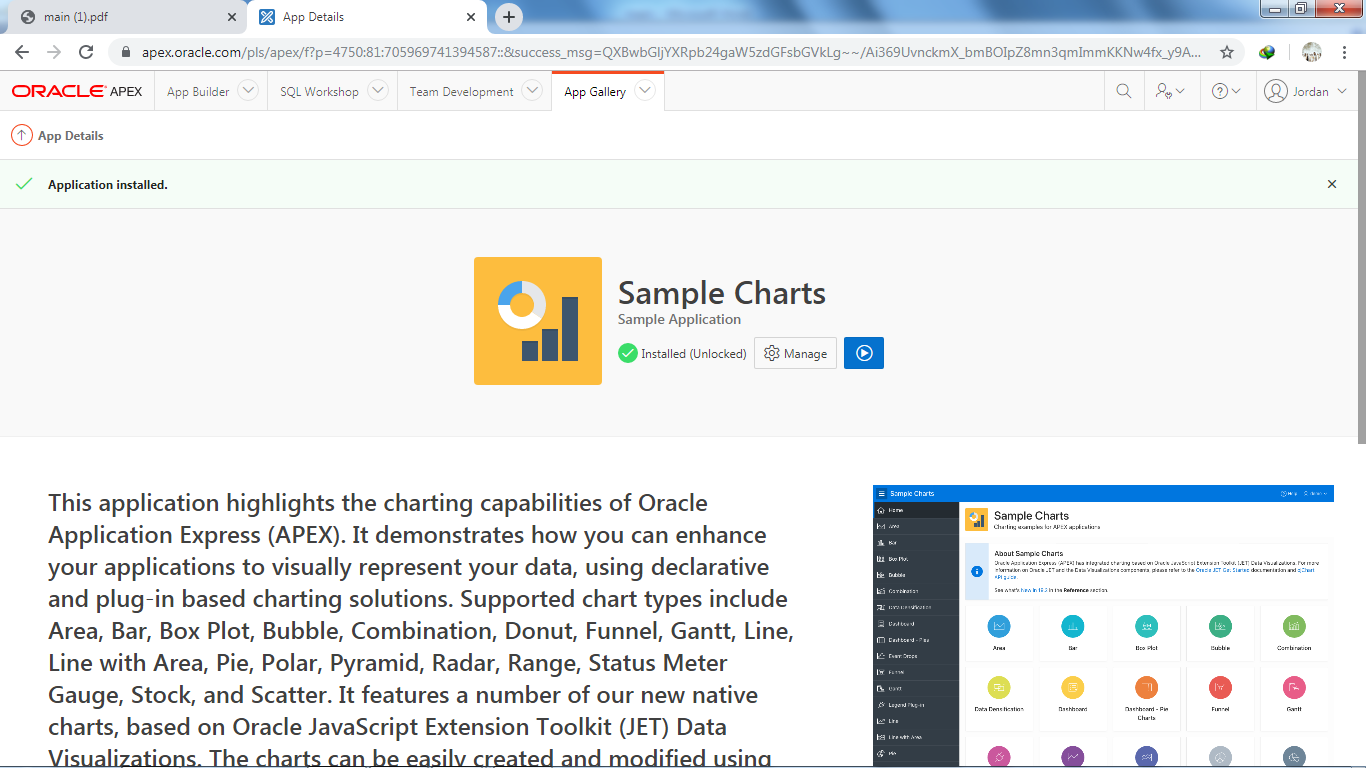
\includegraphics[width=12.5cm]{figures/Screenshot_30.png}
	\caption{App Gallery}
\end{figure}
\item Login ke Aplikasi dan akan masuk ke halaman utama Aplikasi Sample Charts.
\begin{figure}[!htpb]
	\centering
	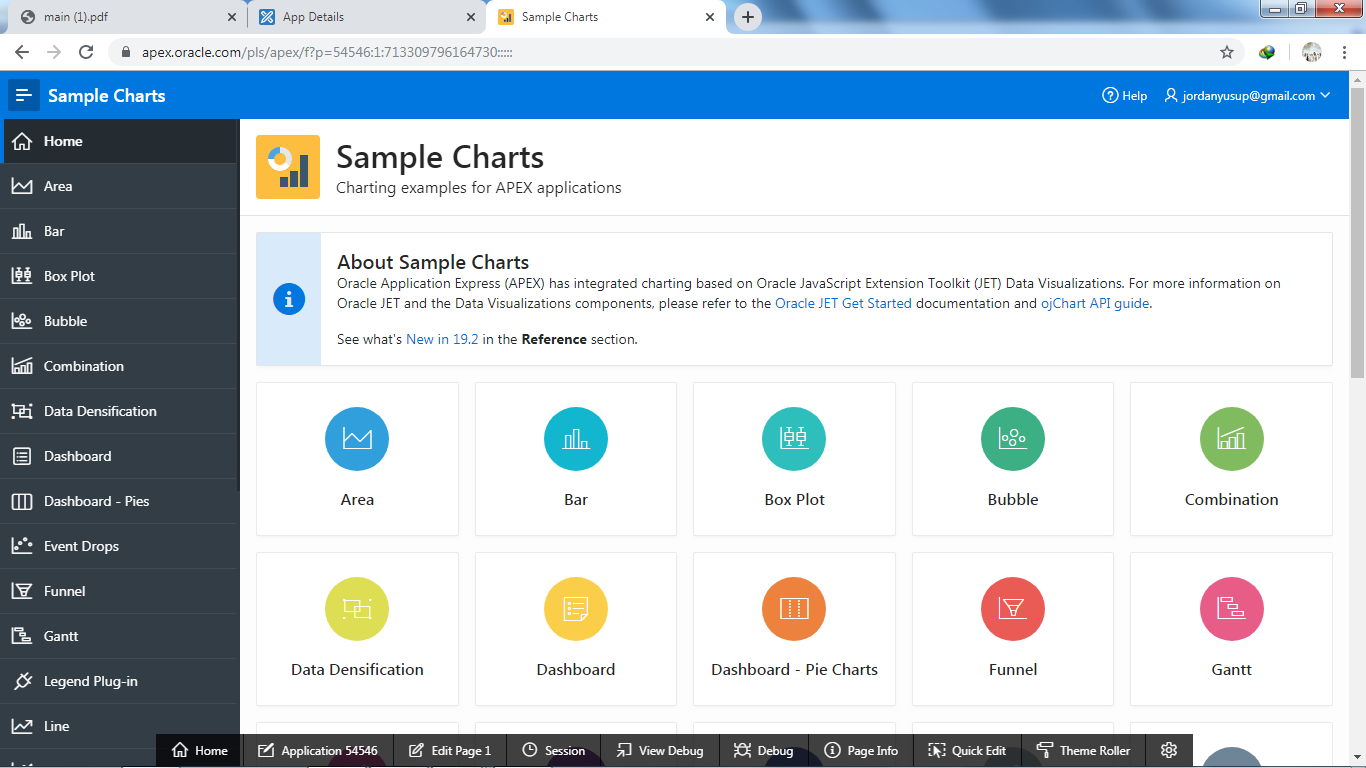
\includegraphics[width=12.5cm]{figures/Screenshot_31.png}
	\caption{App Gallery}
\end{figure}
\end{itemize}
\end{document}

